% Options for packages loaded elsewhere
\PassOptionsToPackage{unicode}{hyperref}
\PassOptionsToPackage{hyphens}{url}
\PassOptionsToPackage{dvipsnames,svgnames,x11names}{xcolor}
%
\documentclass[
  a4paper,
  DIV=11]{scrreprt}

\usepackage{amsmath,amssymb}
\usepackage{iftex}
\ifPDFTeX
  \usepackage[T1]{fontenc}
  \usepackage[utf8]{inputenc}
  \usepackage{textcomp} % provide euro and other symbols
\else % if luatex or xetex
  \usepackage{unicode-math}
  \defaultfontfeatures{Scale=MatchLowercase}
  \defaultfontfeatures[\rmfamily]{Ligatures=TeX,Scale=1}
\fi
\usepackage{lmodern}
\ifPDFTeX\else  
    % xetex/luatex font selection
\fi
% Use upquote if available, for straight quotes in verbatim environments
\IfFileExists{upquote.sty}{\usepackage{upquote}}{}
\IfFileExists{microtype.sty}{% use microtype if available
  \usepackage[]{microtype}
  \UseMicrotypeSet[protrusion]{basicmath} % disable protrusion for tt fonts
}{}
\makeatletter
\@ifundefined{KOMAClassName}{% if non-KOMA class
  \IfFileExists{parskip.sty}{%
    \usepackage{parskip}
  }{% else
    \setlength{\parindent}{0pt}
    \setlength{\parskip}{6pt plus 2pt minus 1pt}}
}{% if KOMA class
  \KOMAoptions{parskip=half}}
\makeatother
\usepackage{xcolor}
\ifLuaTeX
  \usepackage{luacolor}
  \usepackage[soul]{lua-ul}
\else
  \usepackage{soul}
  
\fi
\setlength{\emergencystretch}{3em} % prevent overfull lines
\setcounter{secnumdepth}{5}
% Make \paragraph and \subparagraph free-standing
\ifx\paragraph\undefined\else
  \let\oldparagraph\paragraph
  \renewcommand{\paragraph}[1]{\oldparagraph{#1}\mbox{}}
\fi
\ifx\subparagraph\undefined\else
  \let\oldsubparagraph\subparagraph
  \renewcommand{\subparagraph}[1]{\oldsubparagraph{#1}\mbox{}}
\fi

\usepackage{color}
\usepackage{fancyvrb}
\newcommand{\VerbBar}{|}
\newcommand{\VERB}{\Verb[commandchars=\\\{\}]}
\DefineVerbatimEnvironment{Highlighting}{Verbatim}{commandchars=\\\{\}}
% Add ',fontsize=\small' for more characters per line
\usepackage{framed}
\definecolor{shadecolor}{RGB}{241,243,245}
\newenvironment{Shaded}{\begin{snugshade}}{\end{snugshade}}
\newcommand{\AlertTok}[1]{\textcolor[rgb]{0.68,0.00,0.00}{#1}}
\newcommand{\AnnotationTok}[1]{\textcolor[rgb]{0.37,0.37,0.37}{#1}}
\newcommand{\AttributeTok}[1]{\textcolor[rgb]{0.40,0.45,0.13}{#1}}
\newcommand{\BaseNTok}[1]{\textcolor[rgb]{0.68,0.00,0.00}{#1}}
\newcommand{\BuiltInTok}[1]{\textcolor[rgb]{0.00,0.23,0.31}{#1}}
\newcommand{\CharTok}[1]{\textcolor[rgb]{0.13,0.47,0.30}{#1}}
\newcommand{\CommentTok}[1]{\textcolor[rgb]{0.37,0.37,0.37}{#1}}
\newcommand{\CommentVarTok}[1]{\textcolor[rgb]{0.37,0.37,0.37}{\textit{#1}}}
\newcommand{\ConstantTok}[1]{\textcolor[rgb]{0.56,0.35,0.01}{#1}}
\newcommand{\ControlFlowTok}[1]{\textcolor[rgb]{0.00,0.23,0.31}{#1}}
\newcommand{\DataTypeTok}[1]{\textcolor[rgb]{0.68,0.00,0.00}{#1}}
\newcommand{\DecValTok}[1]{\textcolor[rgb]{0.68,0.00,0.00}{#1}}
\newcommand{\DocumentationTok}[1]{\textcolor[rgb]{0.37,0.37,0.37}{\textit{#1}}}
\newcommand{\ErrorTok}[1]{\textcolor[rgb]{0.68,0.00,0.00}{#1}}
\newcommand{\ExtensionTok}[1]{\textcolor[rgb]{0.00,0.23,0.31}{#1}}
\newcommand{\FloatTok}[1]{\textcolor[rgb]{0.68,0.00,0.00}{#1}}
\newcommand{\FunctionTok}[1]{\textcolor[rgb]{0.28,0.35,0.67}{#1}}
\newcommand{\ImportTok}[1]{\textcolor[rgb]{0.00,0.46,0.62}{#1}}
\newcommand{\InformationTok}[1]{\textcolor[rgb]{0.37,0.37,0.37}{#1}}
\newcommand{\KeywordTok}[1]{\textcolor[rgb]{0.00,0.23,0.31}{#1}}
\newcommand{\NormalTok}[1]{\textcolor[rgb]{0.00,0.23,0.31}{#1}}
\newcommand{\OperatorTok}[1]{\textcolor[rgb]{0.37,0.37,0.37}{#1}}
\newcommand{\OtherTok}[1]{\textcolor[rgb]{0.00,0.23,0.31}{#1}}
\newcommand{\PreprocessorTok}[1]{\textcolor[rgb]{0.68,0.00,0.00}{#1}}
\newcommand{\RegionMarkerTok}[1]{\textcolor[rgb]{0.00,0.23,0.31}{#1}}
\newcommand{\SpecialCharTok}[1]{\textcolor[rgb]{0.37,0.37,0.37}{#1}}
\newcommand{\SpecialStringTok}[1]{\textcolor[rgb]{0.13,0.47,0.30}{#1}}
\newcommand{\StringTok}[1]{\textcolor[rgb]{0.13,0.47,0.30}{#1}}
\newcommand{\VariableTok}[1]{\textcolor[rgb]{0.07,0.07,0.07}{#1}}
\newcommand{\VerbatimStringTok}[1]{\textcolor[rgb]{0.13,0.47,0.30}{#1}}
\newcommand{\WarningTok}[1]{\textcolor[rgb]{0.37,0.37,0.37}{\textit{#1}}}

\providecommand{\tightlist}{%
  \setlength{\itemsep}{0pt}\setlength{\parskip}{0pt}}\usepackage{longtable,booktabs,array}
\usepackage{calc} % for calculating minipage widths
% Correct order of tables after \paragraph or \subparagraph
\usepackage{etoolbox}
\makeatletter
\patchcmd\longtable{\par}{\if@noskipsec\mbox{}\fi\par}{}{}
\makeatother
% Allow footnotes in longtable head/foot
\IfFileExists{footnotehyper.sty}{\usepackage{footnotehyper}}{\usepackage{footnote}}
\makesavenoteenv{longtable}
\usepackage{graphicx}
\makeatletter
\def\maxwidth{\ifdim\Gin@nat@width>\linewidth\linewidth\else\Gin@nat@width\fi}
\def\maxheight{\ifdim\Gin@nat@height>\textheight\textheight\else\Gin@nat@height\fi}
\makeatother
% Scale images if necessary, so that they will not overflow the page
% margins by default, and it is still possible to overwrite the defaults
% using explicit options in \includegraphics[width, height, ...]{}
\setkeys{Gin}{width=\maxwidth,height=\maxheight,keepaspectratio}
% Set default figure placement to htbp
\makeatletter
\def\fps@figure{htbp}
\makeatother
% definitions for citeproc citations
\NewDocumentCommand\citeproctext{}{}
\NewDocumentCommand\citeproc{mm}{%
  \begingroup\def\citeproctext{#2}\cite{#1}\endgroup}
\makeatletter
 % allow citations to break across lines
 \let\@cite@ofmt\@firstofone
 % avoid brackets around text for \cite:
 \def\@biblabel#1{}
 \def\@cite#1#2{{#1\if@tempswa , #2\fi}}
\makeatother
\newlength{\cslhangindent}
\setlength{\cslhangindent}{1.5em}
\newlength{\csllabelwidth}
\setlength{\csllabelwidth}{3em}
\newenvironment{CSLReferences}[2] % #1 hanging-indent, #2 entry-spacing
 {\begin{list}{}{%
  \setlength{\itemindent}{0pt}
  \setlength{\leftmargin}{0pt}
  \setlength{\parsep}{0pt}
  % turn on hanging indent if param 1 is 1
  \ifodd #1
   \setlength{\leftmargin}{\cslhangindent}
   \setlength{\itemindent}{-1\cslhangindent}
  \fi
  % set entry spacing
  \setlength{\itemsep}{#2\baselineskip}}}
 {\end{list}}
\usepackage{calc}
\newcommand{\CSLBlock}[1]{\hfill\break\parbox[t]{\linewidth}{\strut\ignorespaces#1\strut}}
\newcommand{\CSLLeftMargin}[1]{\parbox[t]{\csllabelwidth}{\strut#1\strut}}
\newcommand{\CSLRightInline}[1]{\parbox[t]{\linewidth - \csllabelwidth}{\strut#1\strut}}
\newcommand{\CSLIndent}[1]{\hspace{\cslhangindent}#1}

\usepackage{multicol}
\KOMAoption{captions}{tableheading}
\makeatletter
\@ifpackageloaded{tcolorbox}{}{\usepackage[skins,breakable]{tcolorbox}}
\@ifpackageloaded{fontawesome5}{}{\usepackage{fontawesome5}}
\definecolor{quarto-callout-color}{HTML}{909090}
\definecolor{quarto-callout-note-color}{HTML}{0758E5}
\definecolor{quarto-callout-important-color}{HTML}{CC1914}
\definecolor{quarto-callout-warning-color}{HTML}{EB9113}
\definecolor{quarto-callout-tip-color}{HTML}{00A047}
\definecolor{quarto-callout-caution-color}{HTML}{FC5300}
\definecolor{quarto-callout-color-frame}{HTML}{acacac}
\definecolor{quarto-callout-note-color-frame}{HTML}{4582ec}
\definecolor{quarto-callout-important-color-frame}{HTML}{d9534f}
\definecolor{quarto-callout-warning-color-frame}{HTML}{f0ad4e}
\definecolor{quarto-callout-tip-color-frame}{HTML}{02b875}
\definecolor{quarto-callout-caution-color-frame}{HTML}{fd7e14}
\makeatother
\makeatletter
\@ifpackageloaded{caption}{}{\usepackage{caption}}
\AtBeginDocument{%
\ifdefined\contentsname
  \renewcommand*\contentsname{Inhaltsverzeichnis}
\else
  \newcommand\contentsname{Inhaltsverzeichnis}
\fi
\ifdefined\listfigurename
  \renewcommand*\listfigurename{Abbildungsverzeichnis}
\else
  \newcommand\listfigurename{Abbildungsverzeichnis}
\fi
\ifdefined\listtablename
  \renewcommand*\listtablename{Tabellenverzeichnis}
\else
  \newcommand\listtablename{Tabellenverzeichnis}
\fi
\ifdefined\figurename
  \renewcommand*\figurename{Abbildung}
\else
  \newcommand\figurename{Abbildung}
\fi
\ifdefined\tablename
  \renewcommand*\tablename{Tabelle}
\else
  \newcommand\tablename{Tabelle}
\fi
}
\@ifpackageloaded{float}{}{\usepackage{float}}
\floatstyle{ruled}
\@ifundefined{c@chapter}{\newfloat{codelisting}{h}{lop}}{\newfloat{codelisting}{h}{lop}[chapter]}
\floatname{codelisting}{Listing}
\newcommand*\listoflistings{\listof{codelisting}{Listingverzeichnis}}
\usepackage{amsthm}
\theoremstyle{definition}
\newtheorem{exercise}{Übungsaufgabe}[chapter]
\theoremstyle{definition}
\newtheorem{example}{Beispiel}[chapter]
\theoremstyle{definition}
\newtheorem{definition}{Definition}[chapter]
\theoremstyle{remark}
\AtBeginDocument{\renewcommand*{\proofname}{Beweis}}
\newtheorem*{remark}{Anmerkung}
\newtheorem*{solution}{Lösung}
\newtheorem{refremark}{Anmerkung}[chapter]
\newtheorem{refsolution}{Lösung}[chapter]
\makeatother
\makeatletter
\makeatother
\makeatletter
\@ifpackageloaded{caption}{}{\usepackage{caption}}
\@ifpackageloaded{subcaption}{}{\usepackage{subcaption}}
\makeatother
\ifLuaTeX
\usepackage[bidi=basic]{babel}
\else
\usepackage[bidi=default]{babel}
\fi
\babelprovide[main,import]{ngerman}
% get rid of language-specific shorthands (see #6817):
\let\LanguageShortHands\languageshorthands
\def\languageshorthands#1{}
\ifLuaTeX
  \usepackage{selnolig}  % disable illegal ligatures
\fi
\usepackage{bookmark}

\IfFileExists{xurl.sty}{\usepackage{xurl}}{} % add URL line breaks if available
\urlstyle{same} % disable monospaced font for URLs
\hypersetup{
  pdftitle={Statistik1},
  pdfauthor={Sebastian Sauer},
  pdflang={de},
  colorlinks=true,
  linkcolor={blue},
  filecolor={Maroon},
  citecolor={Blue},
  urlcolor={Blue},
  pdfcreator={LaTeX via pandoc}}

\title{Statistik1}
\author{Sebastian Sauer}
\date{2024-03-05}

\begin{document}
\maketitle

\renewcommand*\contentsname{Inhaltsverzeichnis}
{
\hypersetup{linkcolor=}
\setcounter{tocdepth}{2}
\tableofcontents
}
\chapter{Willkommen!}\label{willkommen}

Statistik und Du: Guter Fit!

\section{Es geht um Ihren Lernerfolg}\label{es-geht-um-ihren-lernerfolg}

Meister Yoda rät: Lesen Sie die Hinweise (Abbildung~\ref{fig-yoda}).

\begin{figure}

\centering{


\includegraphics[width=0.5\textwidth,height=\textheight]{img/yoda.jpg}

}

\caption{\label{fig-yoda}Lesen Sie die folgenden Hinweise im eigenen
Interesse}

\end{figure}%

\href{https://imgflip.com/memegenerator}{Quelle: Imgflip Memengenerator}

\subsection{Lernziele}\label{lernziele}

\begin{itemize}
\item
  Die Studentis sind mit wesentlichen Methoden der explorativen
  Datenanalyse vertraut und können diese selbständig anwenden.
\item
  Die Studentis können gängige Forschungsfragen in lineare Modelle
  übersetzen, diese auf echte Datensätze anwenden und die Ergebnisse
  interpretieren.
\end{itemize}

Kurz gesagt: Das ist ein Grundkurs in Daten zähmen.

\begin{figure}[H]

{\centering 
\includegraphics[width=0.5\textwidth,height=\textheight]{img/datenzaehmen.png}

}

\caption{Daten zähmen}

\end{figure}%

\href{https://github.com/allisonhorst/stats-illustrations}{Bildquelle:
Allison Horst, CC-BY}

\subsection{Was lerne ich hier und wozu ist das
gut?}\label{was-lerne-ich-hier-und-wozu-ist-das-gut}

\emph{Was lerne ich hier?}

Sie lernen das \emph{Handwerk der Datenanalyse} mit einem Schwerpunkt
auf Vorhersage. Anders gesagt: Sie lernen, \emph{Daten aufzubereiten}
und aus Daten \emph{Vorhersagen} abzuleiten. Zum Beispiel: Kommt ein
Student zu Ihnen und sagt ``Ich habe 42 Stunden für die Klausur gelernt,
welche Note kann ich in der Klausur erwarten?''. Darauf Ihre Antwort:
``Auf Basis meiner Daten und meines Modells müsstest du eine 2.7
schreiben!''.\footnote{Darauf dis Studenti: ``Hpmf.''}. Außerdem lernen
Sie, wie man die Güte einer Vorhersage auf Stichhaltigkeit prüft. Denn
Vorhersagen kann man ja in jeder Eckkneipe oder beim Wahrsager bekommen.
Wir wollen aber belastbare Vorhersagen und zumindest wissen, wie gut die
Vorhersagen (von jemanden) bisher waren.

\emph{Warum ist das wichtig?}

Wir wollen nicht auf Leuten vertrauen, die behaupten, sie wüssten, was
für uns richtig und gut ist. Wir wollen selber die Fakten prüfen können.

\emph{Wozu brauche ich das im Job?}

Datenanalyse spielt bereits heute in vielen Berufen eine Rolle. Tendenz
stark zunehmend.

\emph{Wozu brauche ich das im weiterem Studium?}

In Forschungsarbeiten (wie in empirischen Forschungsprojekten, etwa in
der Abschlussarbeit) ist es üblich, statistische Ergebnisse hinsichtlich
quantitativ zu analysieren.

\emph{Ist Statistik nicht sehr abstrakt?}

Der Schwerpunkt dieses Kurses liegt auf Anwenden und Tun; ähnlich dem
Erlernen eines Handwerks. Theorien und Abstraktionen stehen nur am Rand.

\emph{Gibt es auch gute Jobs, wenn man sich mit Daten auskennt?}

Das Forum (2020) berichtet zu den ``Top 20 job roles in increasing and
decreasing demand across industries'' (S. 30, Abb. 22):

\begin{enumerate}
\def\labelenumi{\arabic{enumi}.}
\tightlist
\item
  Data Analysts und Scientists
\item
  AI and Machine Learning Specialists
\item
  Big Data Specialists
\end{enumerate}

\subsection{Motivieren Sie mich!}\label{motivieren-sie-mich}

\href{https://youtu.be/jtNlzpcPr5Y}{Ansprache zur Motivation}

\subsection{Voraussetzungen}\label{voraussetzungen}

Um von diesem Kurs am besten zu profitieren, sollten Sie Folgendes
mitbringen:

\begin{itemize}
\tightlist
\item
  Bereitschaft, Neues zu lernen
\item
  Bereitschaft, nicht gleich aufzugeben
\item
  Kenntnis grundlegender Methoden wissenschaftlichen Arbeitens
\end{itemize}

Was Sie \emph{nicht} brauchen, sind besondere Mathe-Vorkenntnisse.

\subsection{Überblick}\label{uxfcberblick}

Abb. Abbildung~\ref{fig-ueberblick} gibt einen Überblick über den
Verlauf und die Inhalte des Buches. Das Diagramm hilft Ihnen zu
verorten, wo welches Thema im Gesamtzusammenhang steht.

\begin{figure}

\centering{

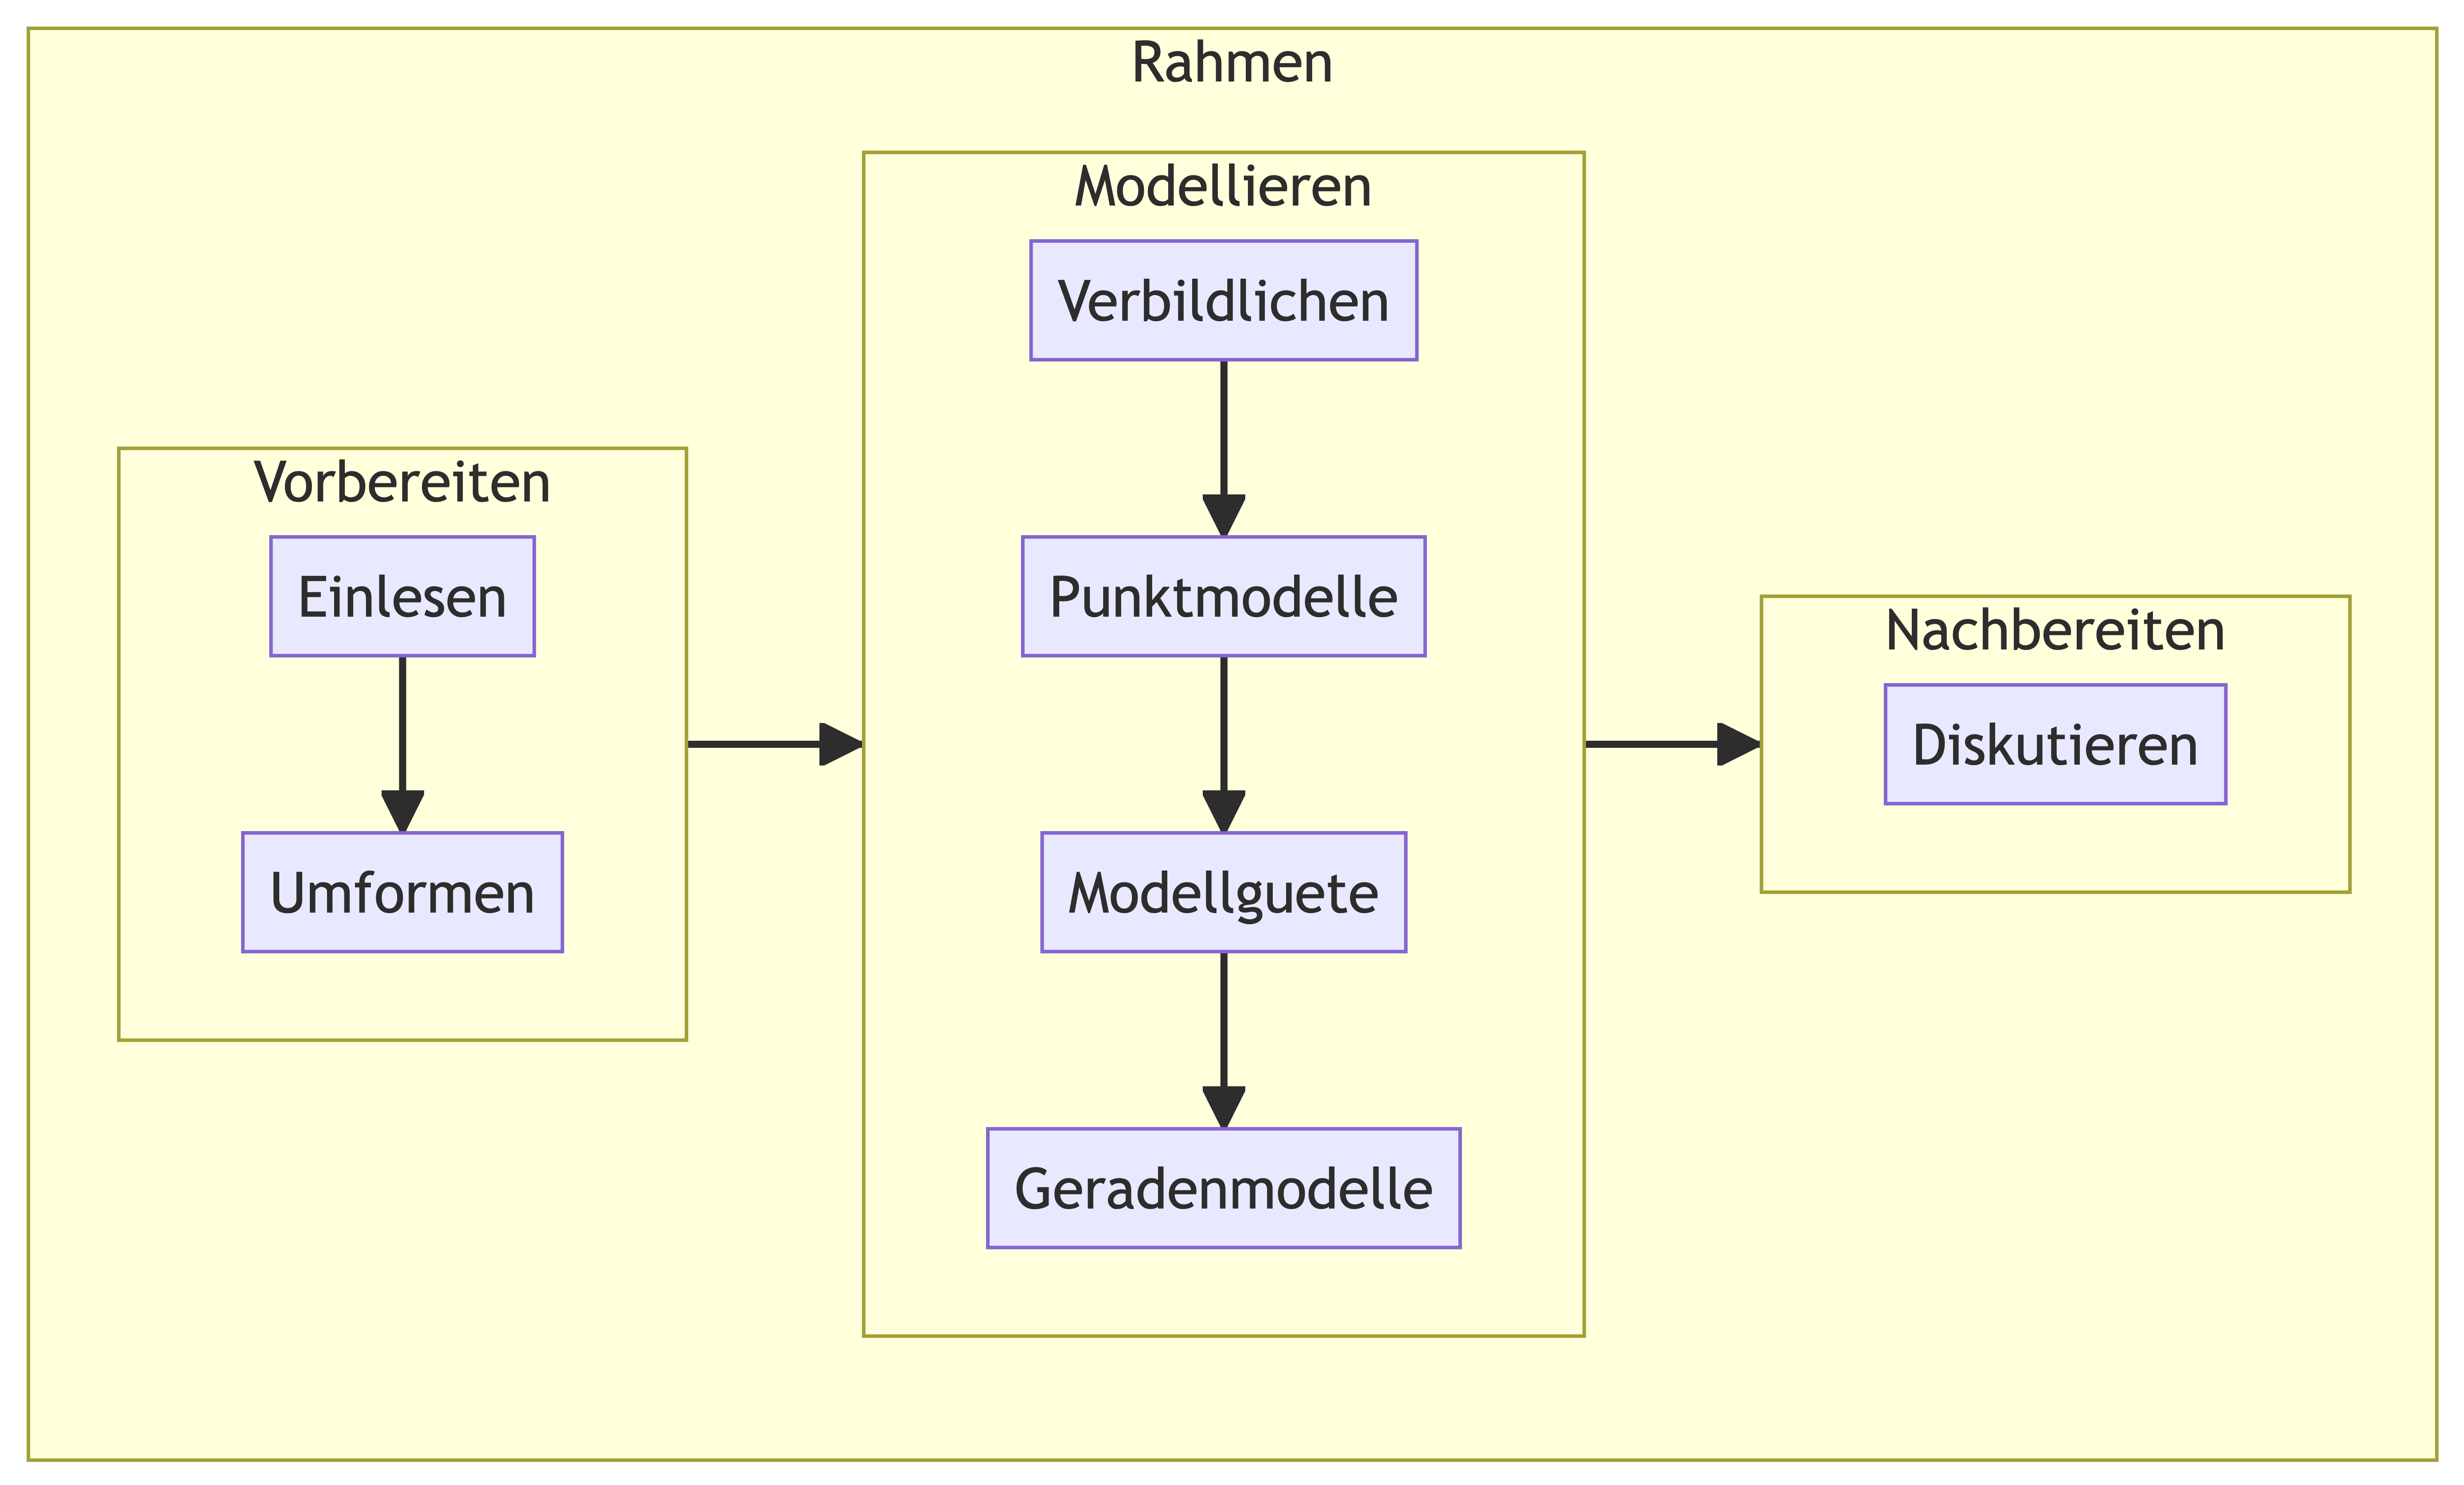
\includegraphics[width=7.24in,height=4.38in]{index_files/figure-latex/mermaid-figure-1.png}

}

\caption{\label{fig-ueberblick}Überblick über den Inhalt und Verlauf des
Buches}

\end{figure}%

Das Diagramm zeigt den Ablauf einer typischen Datenanalyse. Natürlich
kann man sich auch andere sinnvolle Darstellungen dieses Ablaufs
vorstellen.

\subsection{PDF-Version}\label{pdf-version}

Sie können die Druck-Funktion Ihres Broswers nutzen, um ein PDF-Dokument
eines Kapitels dieses Buchs zu erstellen.

\section{Software}\label{software}

Sie benötigen R, RStudio und einige R-Pakete für diesen Kurs.

\subsection{Installation}\label{installation}

\href{https://hinweisbuch.netlify.app/hinweise-software}{Hier} finden
Sie \emph{Installationshinweise.}

\subsection{Viel R (?)}\label{viel-r}

Dieses Buch enthält ``mittel'' viel R. Auf fortgeschrittene R-Techniken
wurde aber komplett verzichtet. Dem einen oder der anderen Anfänger:in
mag es dennoch ``viel Code'' erscheinen. Es wäre ja auch möglich
gewesen, auf R zu verzichten und stattdessen eine ``Klick-Software'' zu
verwenden. \href{https://jasp-stats.org/}{JASP} oder
\href{https://www.jamovi.org/}{Jamovi} sind Beispiele für tolle Software
aus dieser Kategorie. Ich glaube aber, der Verzicht auf eine
Skriptsprache (R) wäre ein schlechter Dienst an den Studentis. Mit Blick
auf eine ``High-Tech-Zukunft'' sollte man zumindest mit etwas
Computer-Code vertraut sein. Auf Computercode zu verzichten erschiene
mir daher fahrlässig für die ``Zukunftsfestigkeit'' der Ausbildung.

\section{Hinweise}\label{hinweise}

\begin{itemize}
\item
  📺
  \href{https://www.youtube.com/channel/UCkvdtj8maE7g-SOCh4aDB9g}{YouTube-Playlists
  zu Statistik}
\item
  \href{https://hinweisbuch.netlify.app/hinweise-lernhilfen-frame}{Lernhilfen}
\item
  \href{https://hinweisbuch.netlify.app/hinweise-didaktik-frame}{Didaktik}
\item
  \href{https://hinweisbuch.netlify.app/hinweise-unterricht-frame}{Unterrichtsorganisation}
\item
  Der Unterricht zu diesem Modul wird nur ein Mal pro Jahr angeboten
  (also nur jedes zweite Semester).
\item
  Eine Prüfung in diesem Modul ist jedes Semester möglich.
\end{itemize}

\section{Prüfung}\label{pruxfcfung}

\href{https://hinweisbuch.netlify.app/hinweise-pruefung-prognosewettbewerb-frame}{Hier}
finden Sie Hinweise zur Prüfung.

\section{Zum Autor}\label{zum-autor}

Nähere Hinweise zum Autor dieses Buch, Sebastian Sauer, finden Sie
\href{https://sebastiansauer-academic.netlify.app/}{hier}.

\section{Nomenklatur}\label{nomenklatur}

\subsection{Griechische Buchstaben}\label{sec-greek}

In diesem Buch werden ein paar (wenige) griechische Buchstaben
verwendet, die in der Statistik üblich sind.

Häufig werden \emph{griechische} Buchstaben verwendet, um eine
Grundgesamtheit (Population) zu beschreiben (die meistens unbekannt
ist). Lateinische (``normale'') Buchstaben werden demgegenüber
verwendet, um eine Stichprobe (Datensatz, vorliegende Daten) zu
beschreiben.

Tabelle~\ref{tbl-griech} stellt diese Buchstaben zusammen mit ihrer
Aussprache und Bedeutung vor.

\begin{longtable}[]{@{}lllr@{}}
\caption{Griechische Buchstaben, die in diesem Buch verwendet
werden.}\label{tbl-griech}\tabularnewline
\toprule\noalign{}
Zeichen & Aussprache & Buchstabe & Bedeutung in der Statistik \\
\midrule\noalign{}
\endfirsthead
\toprule\noalign{}
Zeichen & Aussprache & Buchstabe & Bedeutung in der Statistik \\
\midrule\noalign{}
\endhead
\bottomrule\noalign{}
\endlastfoot
\(\beta\) & beta & b & Regressionskoeffizent \\
\(\mu\) & mü & m & Mittelwert \\
\(\sigma\) & sigma & s & Streuung \\
\(\Sigma\) & Sigma & S & Summenzeichen \\
\(\rho\) & rho & r & Korrelation (nach Pearson) \\
\end{longtable}

Mehr griechische Buchstaben finden sich
\href{https://de.wikipedia.org/wiki/Griechisches_Alphabet}{hier}.

\section{Zitation}\label{zitation}

Bitte zitieren Sie dieses Buch wie folgt:

\begin{quote}
Sauer, S. (2024). \emph{Statistik1}. https://statistik1.netlify.app/
\end{quote}

Hier sind die maschinenlesbaren Zitationsinfos (Bibtex-Format), die Sie
in Ihre Literatursoftware importieren können:

\begin{verbatim}
@book{sauer_statistik1,
    title = {Statistik1},
    rights = {CC-BY-NC},
    url = {https://statistik1.netlify.app/},
    author = {Sauer, Sebastian},
    date = {2024},
}
\end{verbatim}

Hier ist die DOI:

\href{https://zenodo.org/doi/10.5281/zenodo.10082517}{10.5281/zenodo.10082517}

\section{Reproduzierbarkeit}\label{reproduzierbarkeit}

Hier sind einige technische Details zur Reproduzierbarkeit des Buchs.

Dieses Dokument wurde erzeugt am/um 2024-03-04 17:57:04.

\section{Literatur}\label{literatur}

\part{Organisatorisches}

\part{Vorbereiten}

\chapter{Rahmen}\label{rahmen}

\section{Lernsteuerung}\label{lernsteuerung}

\subsection{Standort im Lernpfad}\label{standort-im-lernpfad}

Abbildung~\ref{fig-ueberblick} zeigt den Standort dieses Kapitels im
Lernpfad und gibt damit einen Überblick über das Thema dieses Kapitels
im Kontext aller Kapitel.

Abbildung~\ref{fig-tidy5} zeigt, dass unser Vorgehen in diesem Buch
einem Fließband gleicht: Schritt für Schritt, in der richtigen
Reihenfolge, vom Anfang bis Ende, erarbeiten wir unser ``Datenprodukt''.

\begin{figure}

\centering{

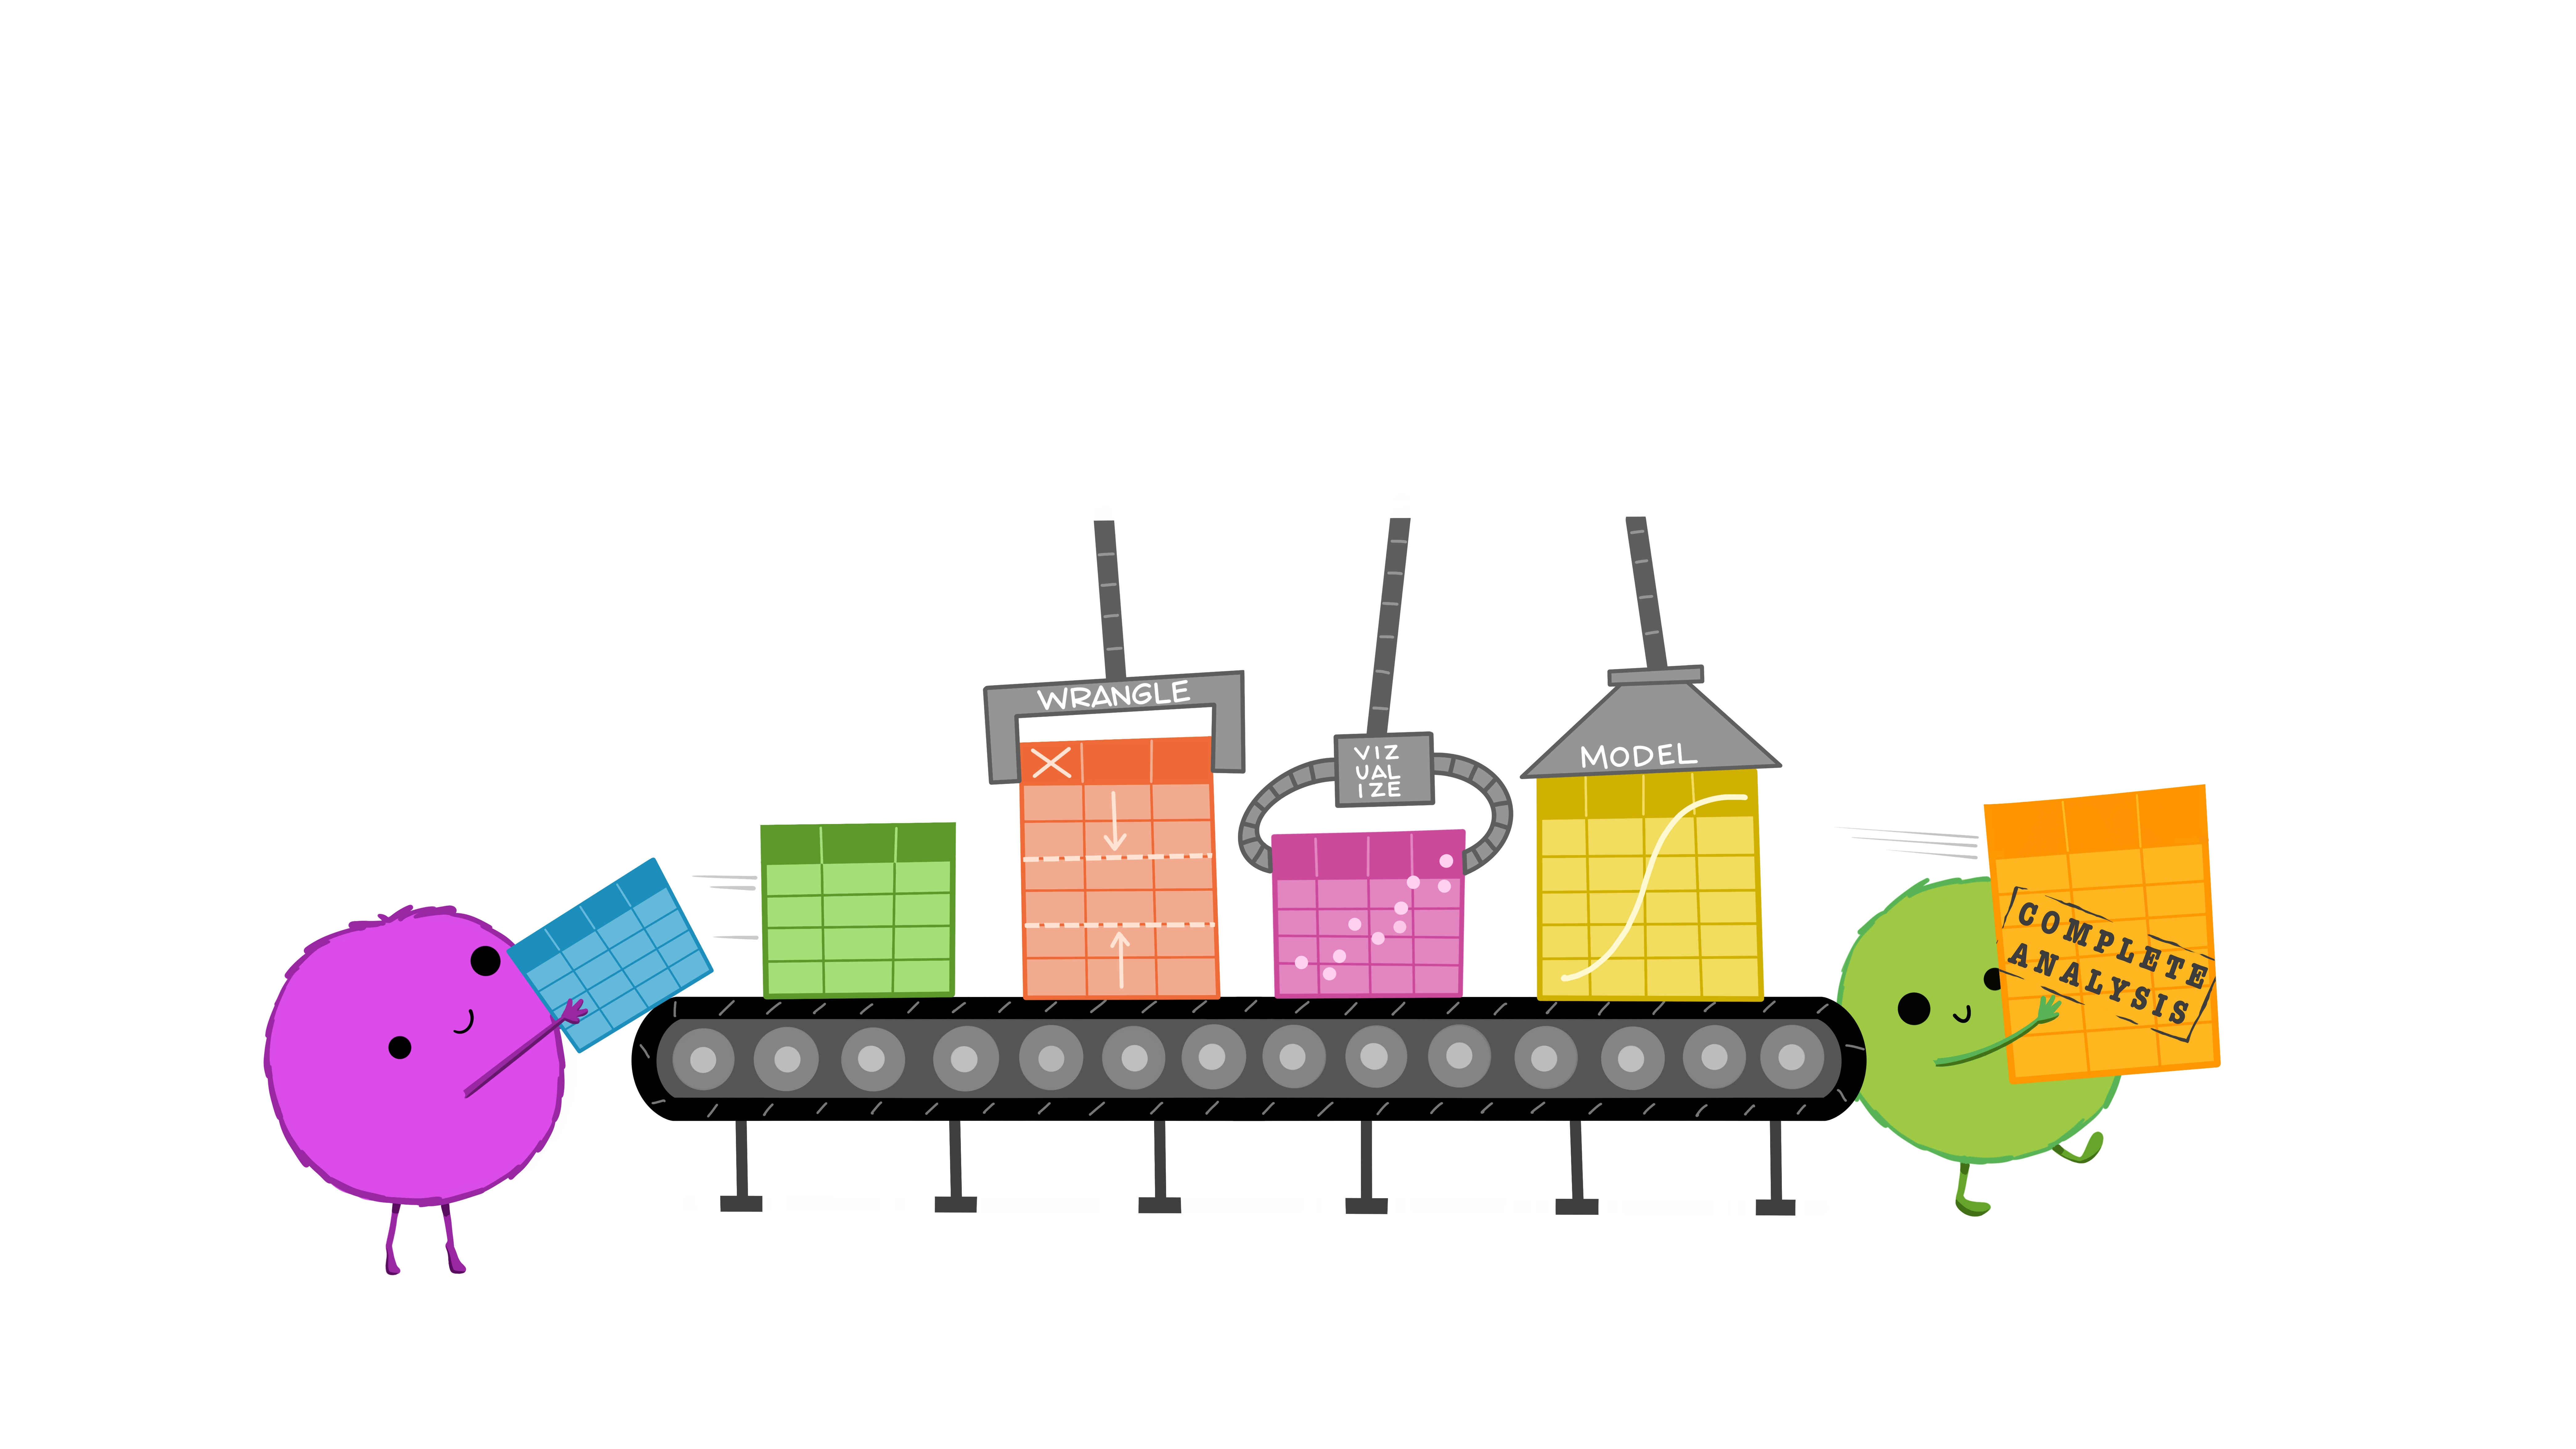
\includegraphics[width=0.75\textwidth,height=\textheight]{img/tidydata_5.jpg}

}

\caption{\label{fig-tidy5}Datenanalyse als eine Abfolge am Fließband}

\end{figure}%

\href{https://github.com/allisonhorst/stats-illustrations}{Quelle}

\subsection{Lernziele}\label{lernziele-1}

\begin{itemize}
\tightlist
\item
  Sie können eine Definition von Statistik wiedergeben.
\item
  Sie können eine Definition von Daten wiedergeben.
\item
  Sie können den Begriff Tidy-Daten erläutern.
\item
  Sie können Beispiele für verschiedene Skalenniveaus nennen.
\end{itemize}

\section{Was ist Statistik und wozu ist sie
gut?}\label{was-ist-statistik-und-wozu-ist-sie-gut}

\subsection{Eine Definition von
Statistik}\label{eine-definition-von-statistik}

Es gibt mehrere Definition von Statistik; hier ist eine.

\begin{definition}[Statistik]\protect\hypertarget{def-statistik}{}\label{def-statistik}

Statistik fasst Daten zusammen, um wesentliche Informationen den Daten
zu entnehmen und beschreibt die Ungewissheit unserer Schlüsse Poldrack
(2023).\(\square\)

\end{definition}

\begin{tcolorbox}[enhanced jigsaw, toptitle=1mm, rightrule=.15mm, colbacktitle=quarto-callout-note-color!10!white, breakable, title=\textcolor{quarto-callout-note-color}{\faInfo}\hspace{0.5em}{Hinweis}, bottomrule=.15mm, colback=white, opacitybacktitle=0.6, left=2mm, titlerule=0mm, toprule=.15mm, coltitle=black, opacityback=0, bottomtitle=1mm, arc=.35mm, leftrule=.75mm, colframe=quarto-callout-note-color-frame]

In diesem Buch werden die Begriffe \emph{Statistik}, \emph{Datenanalyse}
und \emph{Data Science} synonym verwendet.\(\square\)

\end{tcolorbox}

Hm. Vielleicht fragen wir mal ChatGPT, was es unter Statistik versteht:

\begin{quote}
👨 Was ist Statistik? Bitte definiere verständlich.
\end{quote}

\begin{quote}
🤖 Statistik ist eine Wissenschaft, die sich mit der Sammlung, Analyse,
Interpretation, Präsentation und Übertragung von Daten beschäftigt. Ziel
ist es, Muster und Trends in den Daten zu erkennen und verlässliche
Schlussfolgerungen über eine größere Gruppe (z.B. Bevölkerung) auf der
Basis einer Stichprobe (Teilmenge) zu treffen. Die Statistik hilft uns
bei der Beantwortung von Fragen, indem sie uns dabei hilft, die
Unsicherheit in den Daten zu messen und zu verstehen\footnote{Release
  2023-Jan}.
\end{quote}

Gute Antwort, oder?

\begin{exercise}[Nutzen von
Statistik]\protect\hypertarget{exr-nutzen-statistik}{}\label{exr-nutzen-statistik}

🏋️‍♀️ Fragen Sie ChatGPT, was der Nutzen von Statistik ist. Diskutieren Sie
die Antwort.

\end{exercise}

\subsection{Unterschiedlichkeit
messen}\label{unterschiedlichkeit-messen}

Eine allgegenwärtige Tatsache ist, dass die Dinge der Welt sich
unterscheiden, g enauer gesagt, dass Exemplare einer Gattung sich
unterscheiden. So sind nicht alle Menschen gleich groß, nicht alle
Bücher gleich lang oder nicht alle Tage gleich warm.

Ein zentrales Vorgehen bei statistischen Analysen ist es, die
\emph{Unterschiedlichkeit der Dinge} zu beschreiben, präziser gesagt:
die \emph{Variation zu quantifizieren}. Betrachten wir dazu das Beispiel
in s. Abbildung~\ref{fig-groesse}.

\begin{figure}

\centering{

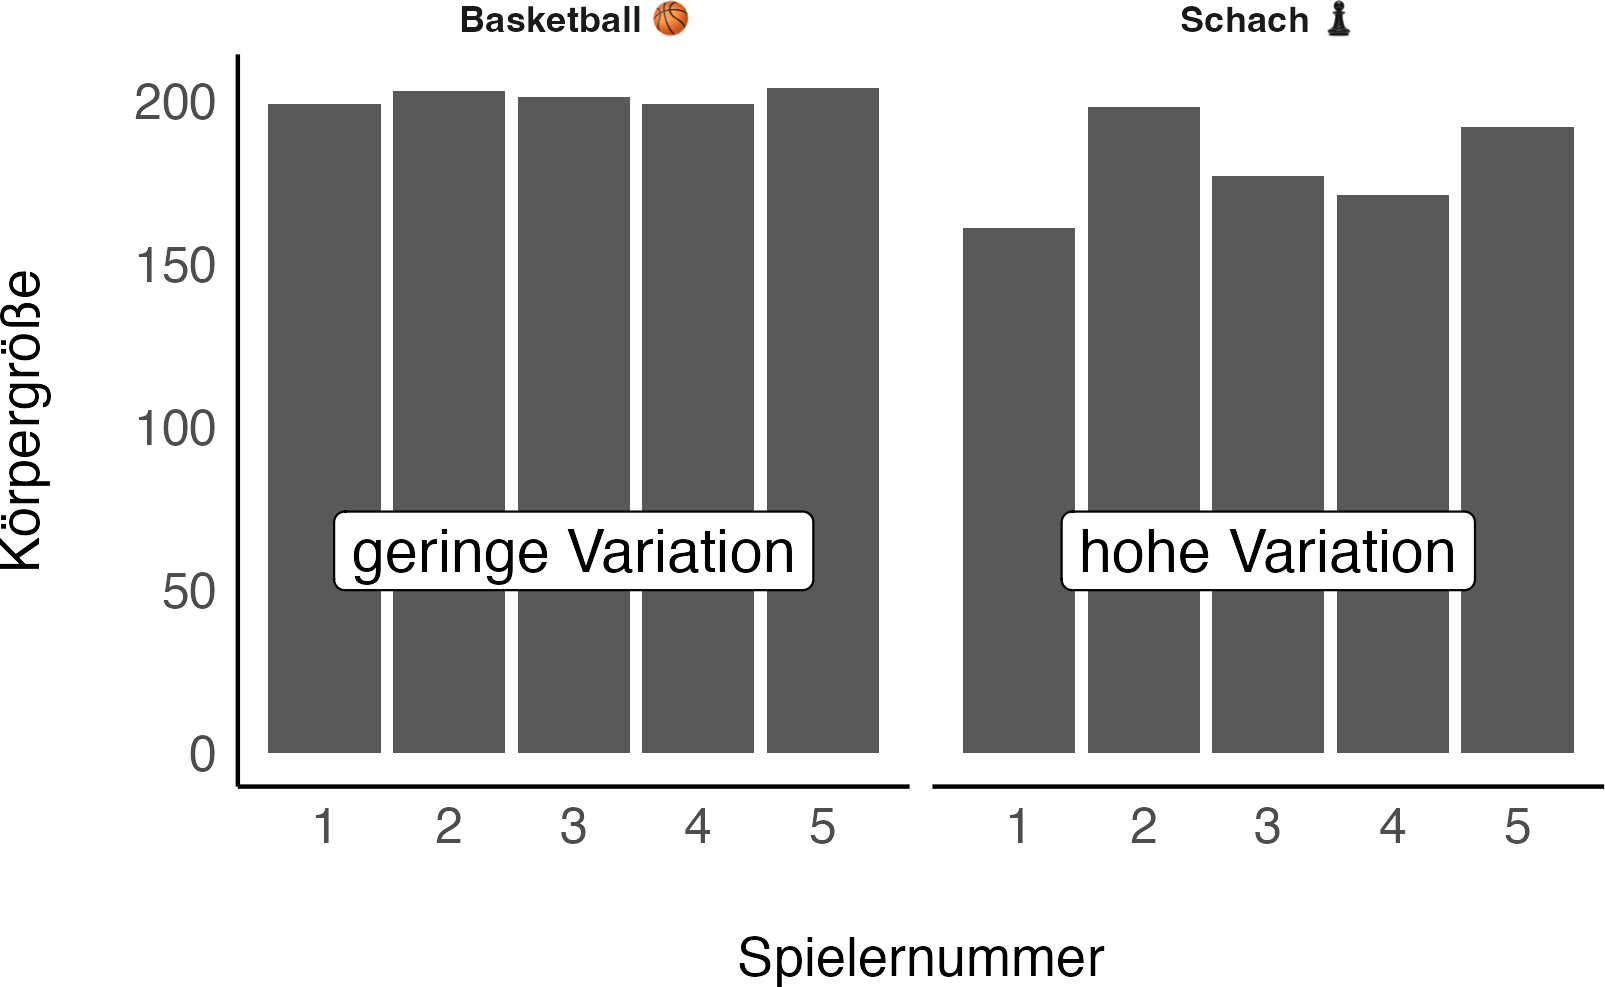
\includegraphics{010-rahmen_files/figure-pdf/fig-groesse-1.png}

}

\caption{\label{fig-groesse}Wenig Variation in der Körpergröße bei den
Basketballern. Alles lange Kerle. Viel Variation bei den Schachspielern:
Manche sind klein, ander groß.}

\end{figure}%

Bei den Basketballern gibt es \emph{geringe} Variation in der
Körpergröße - alle sind groß, ähnlich groß. Bei den Schachspielern gibt
es (im Verhältnis) \emph{hohe} Variation: Einige Personen sind groß,
andere klein.

Die Variation (auch ``Variabilität'' genannt) kann man auch gut so
darstellen wie in s. Abbildung~\ref{fig-variab} gezeigt.

\begin{figure}

\centering{

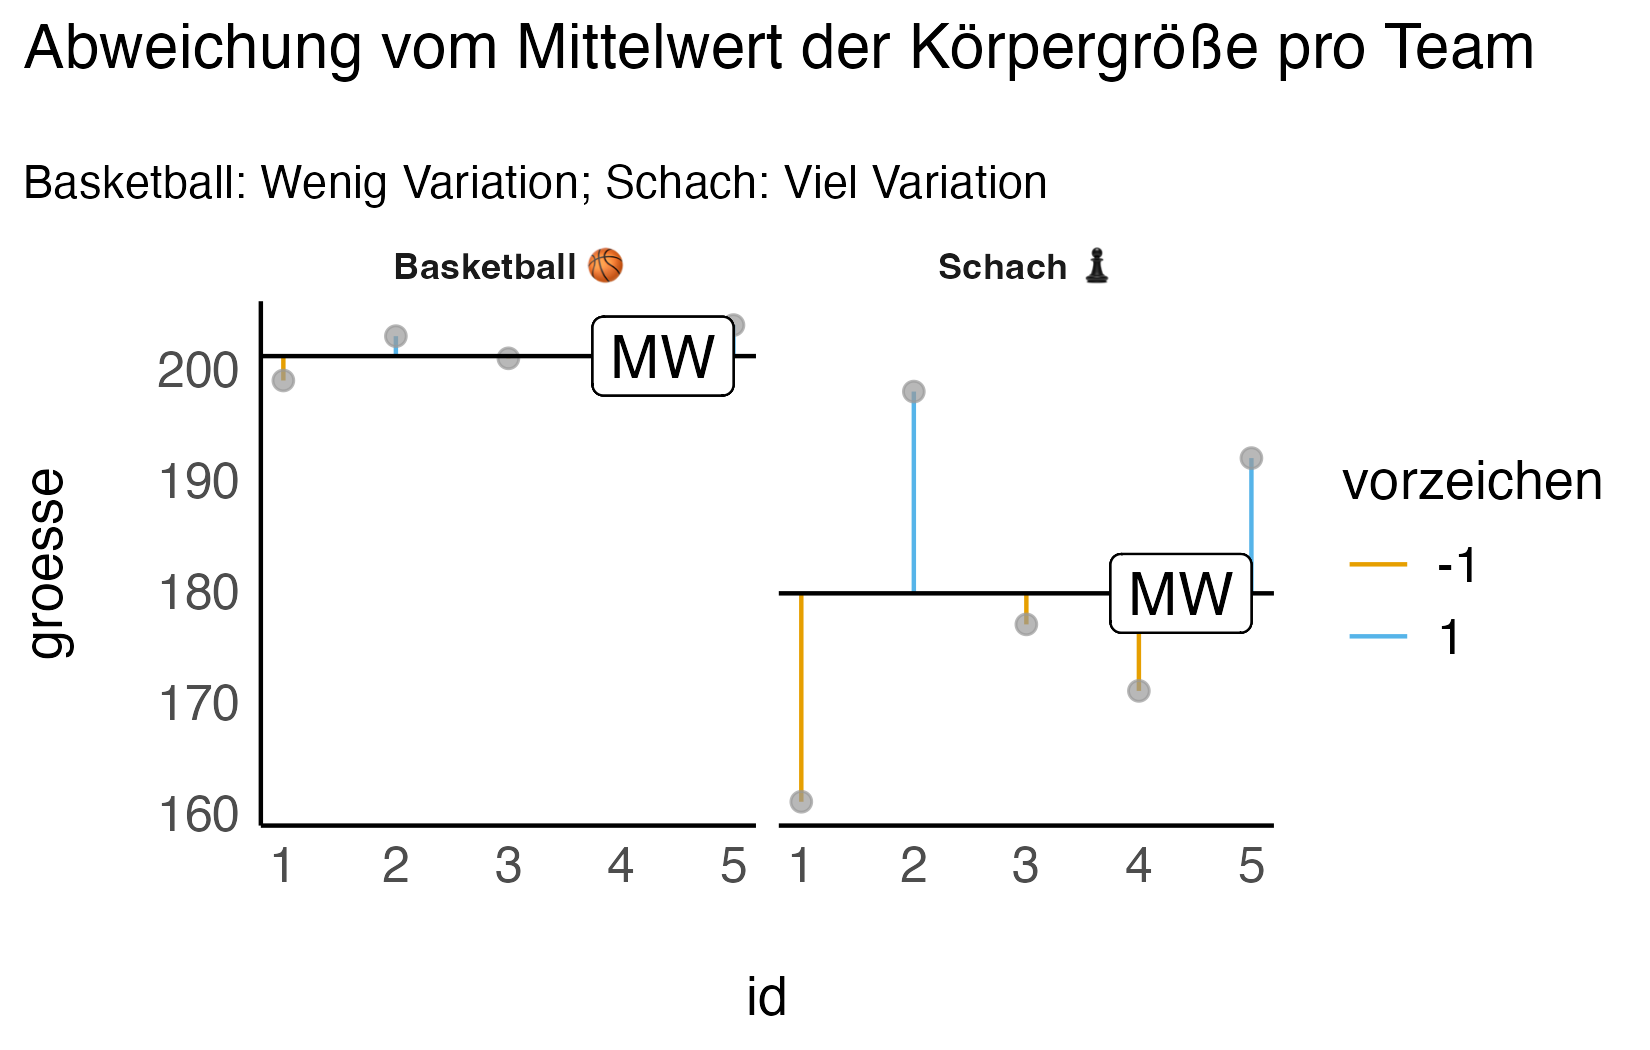
\includegraphics{010-rahmen_files/figure-pdf/fig-variab-1.png}

}

\caption{\label{fig-variab}Die Abweichungen der einzelnen Personen von
der mittleren Körpergröße ihres Teams}

\end{figure}%

Eine \emph{Abweichung} (auch \emph{Residuum}) genannt, zeigt hier die
Differenz von Mittelwert und dem Wert der Körpergröße bei der jeweiligen
Person. Wenn wir allgemein von einer Person \(i\) sprechen, Das Merkmal
\emph{Körpergröße} mit \(X\) bezeichnen und den Mittelwert der
Körpergröße als \(\bar{x}\) (``x quer''), dann können wir knapp und
präzise das Residuum der \(i\)-ten Person mit \(r_i\) bezeichnen und
entsprechend definieren.

\begin{definition}[Residuum]\protect\hypertarget{def-residuum}{}\label{def-residuum}

Das Residuum des Merkmals \(X\) der \(i\)-ten Beobachtung ist definiert
als die Differenz vom Wert \(x_i\) und einem Referenzwert, etwa dem
Mittelwert, \(\bar{x}\):

\(r_i = x_i - \bar{x}\). \(\square\)

\end{definition}

\section{Was ist das Ziel Ihrer
Analyse?}\label{was-ist-das-ziel-ihrer-analyse}

\subsection{Arten von Zielen}\label{arten-von-zielen}

\begin{figure}

\centering{

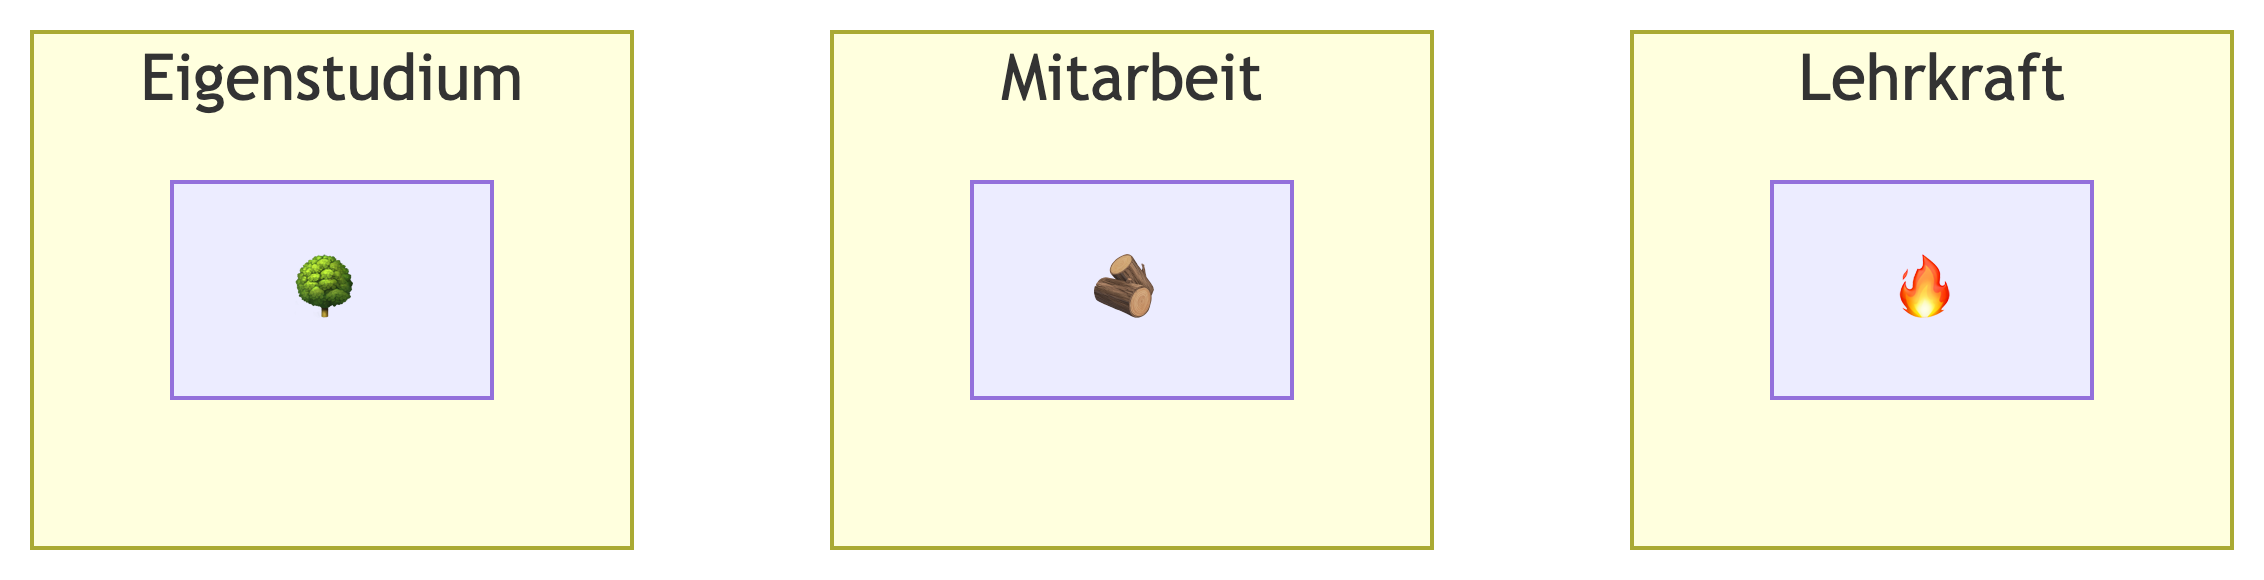
\includegraphics[width=4.84in,height=1.04in]{010-rahmen_files/figure-latex/mermaid-figure-1.png}

}

\caption{\label{fig-ziele}Zielarten einer Datenanalyse}

\end{figure}%

Beispiele für die einzelnen Zielarten der Datenanalyse:

\begin{itemize}
\tightlist
\item
  \emph{Beschreiben}: ``Wie groß ist der Gender-Paygap in der Branche X
  im Zeitraum Y?''
\item
  \emph{Vorhersagen}: Wenn ich 100 Stunden auf die Statistikklausur
  lernen, welche Note kann ich dann erwarten?
\item
  \emph{Erklären}: Wie viel bringt mir das Lernen auf die
  Statistikklausur?
\end{itemize}

\subsection{Forschungsfrage}\label{forschungsfrage}

Eine Forschungsfrage ist die Leitfrage Ihrer Analyse. Sie definiert, was
Sie herausfinden wollen. Häufig sind Forschungsfragen so aufgebaut:

\begin{quote}
Hat X einen Einfluss auf Y?
\end{quote}

Eine Forschungsfrage weist häufig folgende Struktur auf, s.
Abbildung~\ref{fig-fo-struktur}.

\begin{figure}

\centering{

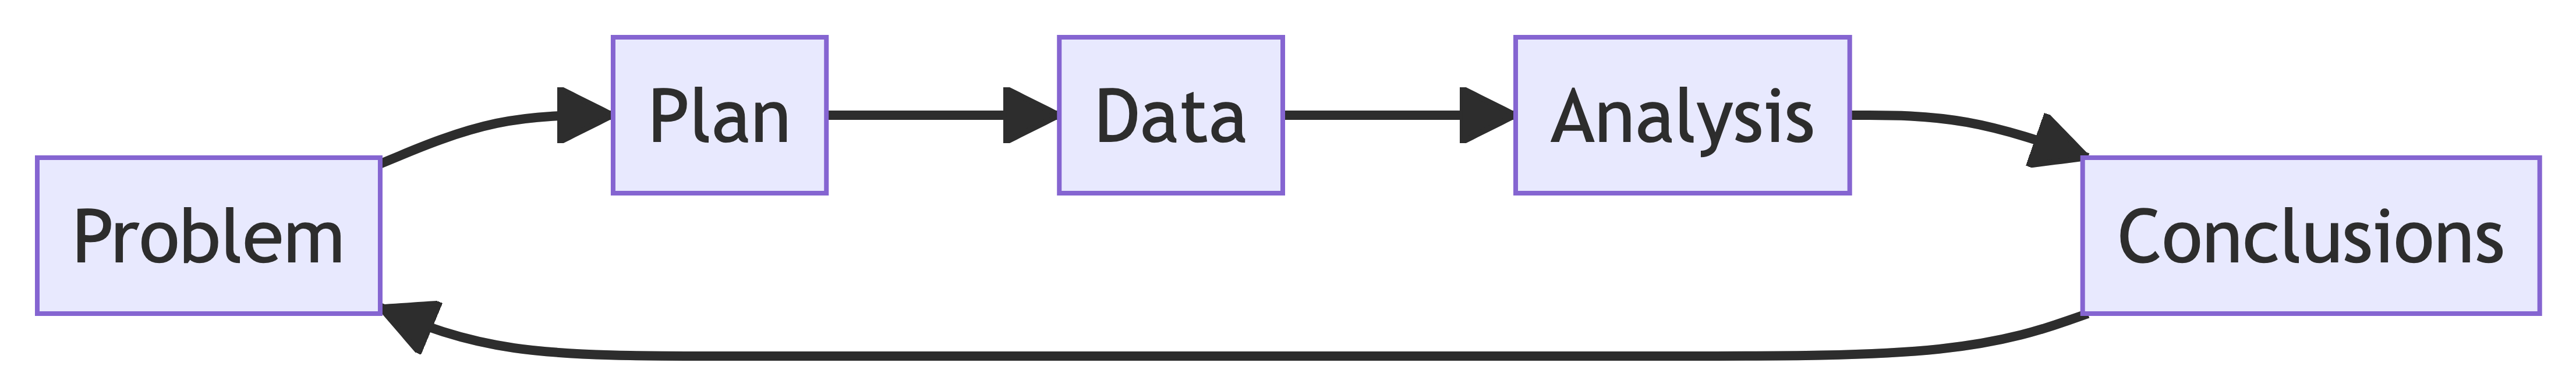
\includegraphics[width=4.83in,height=1.24in]{010-rahmen_files/figure-latex/mermaid-figure-4.png}

}

\caption{\label{fig-fo-struktur}Struktur eine Forschungsfrage}

\end{figure}%

\begin{example}[Forschungsfrage
1]\protect\hypertarget{exm-fofrage1}{}\label{exm-fofrage1}

~

\begin{quote}
Hat Lernen einen Einfluss auf den Prüfungserfolg? Verringert Joggen die
Menge des Hüftgolds? Um welchen Betrag erhöht sich der Umsatz, wenn wir
1000€ mehr Werbung ausgeben?\(\square\)
\end{quote}

\end{example}

\begin{example}[Forschungsfrage
2]\protect\hypertarget{exm-fofrage2}{}\label{exm-fofrage2}

Nach dem Studium haben Sie bei einem großen Online-Auktionshaus
angeheuert. Da Sie angaben, sich im Studium \st{intensiv} etwas mit
Statistik beschäftigt zu haben, hat man Sie in die
F\&E-Abteilung\footnote{Forschung und Entwicklung} gesteckt. Heute ist
es Ihre Aufgabe, Auktionen zur Spielekonsole
\href{https://www.nintendo.de/Wii/Wii-94559.html}{Wii} zu untersuchen,
genauer gesagt, geht es um das Spiel
\href{https://www.nintendo.de/Spiele/Wii/Mario-Kart-Wii-281848.html\#_bersicht}{Mariokart}.
Ihre Forschungsfrage lautet:

\begin{quote}
Welche Produktmerkmale stehen mit einem hohen Verkaufserlös in
Zusammenhang?\(\square\)
\end{quote}

\end{example}

\begin{example}[Aus der Forschung: Smartphone-Brain-Drain
📱🧠🚫]\protect\hypertarget{exm-braindrain}{}\label{exm-braindrain}

Ward et al. (2017) untersuchten die Forschungsfrage, ob die bloße
Gegenwart eines Handies (z.B. wenn es vor Ihnen auf dem Tisch liegt)
dazu führt, dass man abgelenkt wird und daher schlechtere kognitive
Leistungen zeigt.

Leider schreiben die Autoren Ihre Hypothese nicht glasklar, aber
implizit ist obige Hypothese herauszulesen:

\begin{quote}
First, smartphones may redirect the orientation of conscious attention
away from the focal task and toward thoughts or behaviors associated
with one's phone. Prior research provides ample evidence that \ldots{}
this digital distraction adversely affects both performance \ldots{} and
enjoyment.
\end{quote}

Später formulieren Sie Ihre Hypothese noch genauer:

\begin{quote}
In two experiments, we test the hypothesis that the mere presence of
one's own smartphone reduces available cognitive capacity.
\end{quote}

Die Ergebnisse unterstützen Ihre Hypothese, s.
Abbildung~\ref{fig-braindrain}. Im Diagramm ist ersichtlich, dass die
kognitive Leistung (Y-Achse) sowohl in der Kapazität des
Arbeitsgedächtnisses (links) als auch in der fluiden Intelligenz
(rechts) am geringsten ist, wenn das Handy auf dem Schreibtisch (Desk)
liegt. Am besten ist die kognitive Leistung, wenn das Handy nicht im
Raum ist.\(\square\)

\begin{figure}

\centering{

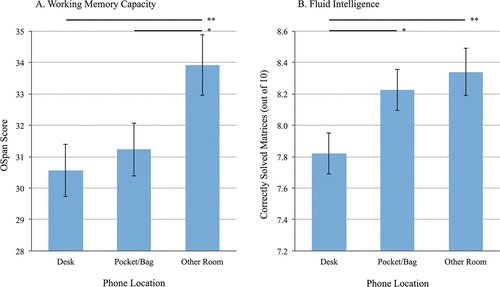
\includegraphics{img/braindrain1.jpg}

}

\caption{\label{fig-braindrain}Handy in Sichtweite verringert die
kognitiven Ressourcen}

\end{figure}%

\end{example}

\begin{tcolorbox}[enhanced jigsaw, toptitle=1mm, rightrule=.15mm, colbacktitle=quarto-callout-caution-color!10!white, breakable, title=\textcolor{quarto-callout-caution-color}{\faFire}\hspace{0.5em}{Vorsicht}, bottomrule=.15mm, colback=white, opacitybacktitle=0.6, left=2mm, titlerule=0mm, toprule=.15mm, coltitle=black, opacityback=0, bottomtitle=1mm, arc=.35mm, leftrule=.75mm, colframe=quarto-callout-caution-color-frame]

Es ist ein häufiger Fehler, in der Forschungsfrage zu formulieren ``X
führt zu Y'', aber in der Analyse keine Methode zu verwenden, die
geeignet ist, kausale Zusammenhänge aufzudecken. Es reicht nicht, dass
man z.B. einen (negativen) Zusammenhang zwischen der Häufigkeit von
Smartphone-Nutzung und Konzentrationsfähigkeit findet (Schwaiger \&
Tahir, 2022), um zu sagen: ``Daddeln macht dumm!''. Es könnte ja z.B.
auch umgekehrt sein. Platt gesagt: ``Dummheit führt zu Daddeln''.
Weitere Erklärungen sind möglich. Vorsicht also mit (vor)schnellen
Aussagen zu kausalen Abhängigkeiten.

\end{tcolorbox}

\section{Was sind Daten?}\label{was-sind-daten}

\begin{definition}[Hallo,
Daten]\protect\hypertarget{def-daten}{}\label{def-daten}

Daten kann man als eine geordnete Folge von Zeichen
definieren.\(\square\)

\end{definition}

Daten kommen häufig in Tabellenform vor; so sind sie (oft) am besten zu
untersuchen, s. Tabelle~\ref{tbl-daten}.

\begin{longtable}{rlr}

\caption{\label{tbl-daten}So sehen Daten aus.}

\tabularnewline

\toprule
id & name & note \\ 
\midrule\addlinespace[2.5pt]
1 & Anna & 1.3 \\ 
2 & Berta & 2.3 \\ 
3 & Carla & 3.0 \\ 
\bottomrule

\end{longtable}

Die erste Spalte \texttt{id} ist nur eine laufende Nummer. Sie dient
dazu, die einzelnen Beobachtungen (hier Studentis) identifizieren zu
können und birgt ansonsten keine Information. Beispiele für ID-Variablen
sind z.B. Matrikulationsnummer, Personalausweisnummern oder
Bestellnummern.

\subsection{Je mehr, desto besser (?)}\label{je-mehr-desto-besser}

Was Daten betrifft, könnte man behaupten: ``Viel hilft viel'' oder ``Je
mehr, desto besser''. Natürlich unter sonst gleichen
Umständen\footnote{Ceteris paribus, auf Latein, hört sich gleich viel
  schlauer an}. Viel Datenmüll ist natürlich nicht besser als ein paar
knappe, wasserdichte Fakten!

\begin{example}[]\protect\hypertarget{exm-samplesize}{}\label{exm-samplesize}

Um Ihre eigene Lehraktivität zu organisieren, wollen Sie sich ein Bild
machen, wie viel Ihre Nebensitzer im Hörsaal so lernen. Sie blicken nach
links und fragen ``wie viel lernst du so?''. Sie blicken nach recht und
wiederholen die Frage gerichtet an den rechtsnebensitzenden
Kommilitonen. Dann addieren Sie die zwei Zahlen (unter der Annahme, dass
Sie zwei Zahlen bekommen haben), und teilen durch zwei, um den
Mittelwert zu erhalten.

Ein kritischer Geist könnte anmerken, dass Sie besser die Untersuchung
nicht gemacht hätten (auch wenn Sie, vielleicht ohne zu wollen, eine
statistische Untersuchung angestellt haben). Denn bei so wenig befragten
Personen ist die Ungenauigkeit Ihrer Schätzung der typischen Lernzeit
bei Studentis einfach zu hoch.\(\square\)

\end{example}

Abbildung~\ref{fig-sample-estimate} veranschaulicht, dass man einen
Mittelwert genauer schätzen kann, wenn man auf eine größere Stichprobe
zurückgreift. Das Teilbild links zeigt den Mittelwert einer Stichprobe
mit \(n=20\) Beobachtungen. Das Teilbild rechts zeigt den Mittelwert
einer Stichprobe mit \(n=200\) Beobachtungen (jeweils aus der gleichen
Grundgesamtheit). Wie man sieht, ist im linken Teilbild die Streuung
(Variation) höher als im rechten Teilbild:

\begin{verbatim}
## $x
## [1] "Nummer der Stichprobe"
## 
## $y
## [1] "Wert"
## 
## attr(,"class")
## [1] "labels"
\end{verbatim}

\begin{figure}

\centering{

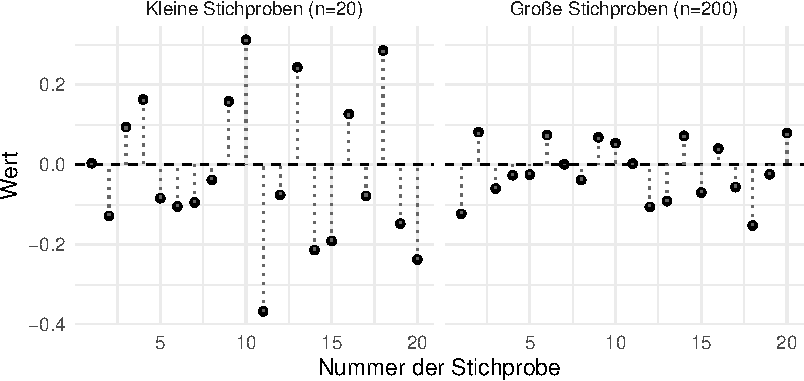
\includegraphics{010-rahmen_files/figure-pdf/fig-sample-estimate-1.pdf}

}

\caption{\label{fig-sample-estimate}Schätzgenauigkeit als Funktion der
Stichprobengröße}

\end{figure}%

Bildquelle: Karsten Lübke

\begin{tcolorbox}[enhanced jigsaw, toptitle=1mm, rightrule=.15mm, colbacktitle=quarto-callout-important-color!10!white, breakable, title=\textcolor{quarto-callout-important-color}{\faExclamation}\hspace{0.5em}{Wichtig}, bottomrule=.15mm, colback=white, opacitybacktitle=0.6, left=2mm, titlerule=0mm, toprule=.15mm, coltitle=black, opacityback=0, bottomtitle=1mm, arc=.35mm, leftrule=.75mm, colframe=quarto-callout-important-color-frame]

Mehr Daten = genauere Ergebnisse (unter sonst gleichen Umständen)
\(\square\)

\end{tcolorbox}

\begin{example}[Daten zur Forschungsfrage
2]\protect\hypertarget{exm-daten}{}\label{exm-daten}

Hier ist ein Auszug der Daten zur Tabelle \texttt{mariokart}, s.
Tabelle~\ref{tbl-mariokart}.

\begin{longtable}[]{@{}
  >{\raggedleft\arraybackslash}p{(\columnwidth - 18\tabcolsep) * \real{0.1011}}
  >{\raggedleft\arraybackslash}p{(\columnwidth - 18\tabcolsep) * \real{0.0787}}
  >{\raggedright\arraybackslash}p{(\columnwidth - 18\tabcolsep) * \real{0.0562}}
  >{\raggedleft\arraybackslash}p{(\columnwidth - 18\tabcolsep) * \real{0.1011}}
  >{\raggedleft\arraybackslash}p{(\columnwidth - 18\tabcolsep) * \real{0.0899}}
  >{\raggedleft\arraybackslash}p{(\columnwidth - 18\tabcolsep) * \real{0.1011}}
  >{\raggedright\arraybackslash}p{(\columnwidth - 18\tabcolsep) * \real{0.1236}}
  >{\raggedleft\arraybackslash}p{(\columnwidth - 18\tabcolsep) * \real{0.1348}}
  >{\raggedright\arraybackslash}p{(\columnwidth - 18\tabcolsep) * \real{0.1348}}
  >{\raggedleft\arraybackslash}p{(\columnwidth - 18\tabcolsep) * \real{0.0787}}@{}}

\caption{\label{tbl-mariokart}Auszug aus der Tabelle mariokart}

\tabularnewline

\toprule\noalign{}
\begin{minipage}[b]{\linewidth}\raggedleft
duration
\end{minipage} & \begin{minipage}[b]{\linewidth}\raggedleft
n\_bids
\end{minipage} & \begin{minipage}[b]{\linewidth}\raggedright
cond
\end{minipage} & \begin{minipage}[b]{\linewidth}\raggedleft
start\_pr
\end{minipage} & \begin{minipage}[b]{\linewidth}\raggedleft
ship\_pr
\end{minipage} & \begin{minipage}[b]{\linewidth}\raggedleft
total\_pr
\end{minipage} & \begin{minipage}[b]{\linewidth}\raggedright
ship\_sp
\end{minipage} & \begin{minipage}[b]{\linewidth}\raggedleft
seller\_rate
\end{minipage} & \begin{minipage}[b]{\linewidth}\raggedright
stock\_photo
\end{minipage} & \begin{minipage}[b]{\linewidth}\raggedleft
wheels
\end{minipage} \\
\midrule\noalign{}
\endhead
\bottomrule\noalign{}
\endlastfoot
3 & 20 & new & 0.99 & 4.00 & 51.55 & standard & 1580 & yes & 1 \\
7 & 13 & used & 0.99 & 3.99 & 37.04 & firstClass & 365 & yes & 1 \\
3 & 16 & new & 0.99 & 3.50 & 45.50 & firstClass & 998 & no & 1 \\
3 & 18 & new & 0.99 & 0.00 & 44.00 & standard & 7 & yes & 1 \\
1 & 20 & new & 0.01 & 0.00 & 71.00 & media & 820 & yes & 2 \\
3 & 19 & new & 0.99 & 4.00 & 45.00 & standard & 270144 & yes & 0 \\

\end{longtable}

Eine Erklärung aller Variablen des Datensatzes \texttt{mariokart} findet
sich
\href{https://www.openintro.org/data/index.php?data=mariokart}{hier}.
\(\square\)

\end{example}

\begin{definition}[Data
Dictionary]\protect\hypertarget{def-datadict}{}\label{def-datadict}

Eine Erklärung, was die Namen einer Datentabelle bedeuten, nennt man
\emph{Code Book} or \emph{Data Dictionary}.\(\square\)

\end{definition}

\begin{tcolorbox}[enhanced jigsaw, toptitle=1mm, rightrule=.15mm, colbacktitle=quarto-callout-note-color!10!white, breakable, title=\textcolor{quarto-callout-note-color}{\faInfo}\hspace{0.5em}{Wie man mit Statistik lügt: Das File-Drawer-Problem}, bottomrule=.15mm, colback=white, opacitybacktitle=0.6, left=2mm, titlerule=0mm, toprule=.15mm, coltitle=black, opacityback=0, bottomtitle=1mm, arc=.35mm, leftrule=.75mm, colframe=quarto-callout-note-color-frame]

Sie haben ein tolles Experiment durchgeführt, viel Arbeit, viel Stress,
endlich geschafft, puh. Von den 20 Variablen (als AV, s.
Kapitel~\ref{sec-arten-variablen}), die Sie untersucht haben, zeigt nur
1 einen interessanten Effekt, leider. 1 von 20, das hört sich nicht so
toll an. Wäre es da nicht ``elegant'', die 19 Variablen ohne schönen
Effekt einfach in der Schublade liegen zu lassen bis zum
Sankt-Nimmerleins-Tag? Dann könnten Sie stattdessen als Ergebnis nur die
eine Variable mit schönen Ergebnis präsentieren, ganz ohne
widersprechende Befunde.

Dieser Versuchung nicht zu erliegen, kann schwer sein. Es ist aber
gefährlich, missliebige Ergebnisse zu verschweigen: Die anderen Menschen
bekommen dann ein falsches Bild der Ergebnislage; man spricht von
\href{https://de.wikipedia.org/wiki/Publikationsbias}{Publikationsbias}.
Wer Ergebnisse verschweig, verzerrt die insgesamte Befundlage
(Rothstein, 2014).

\end{tcolorbox}

\subsection{Was ist eine Variable?}\label{was-ist-eine-variable}

\begin{definition}[Variable]\protect\hypertarget{def-var}{}\label{def-var}

Eine Variable ist ein Platzhalter, der für ein Merkmal steht, das
verschiedene Werte annehmen kann.\(\square\)

\end{definition}

Man kann sich eine Variable wie einen Behälter vorstellen, auf dem mit
einem Stift geschrieben steht, was für eine Art Inhalt darin ist, s.
Abbildung~\ref{fig-var-zuweisen}.

\begin{figure}

\centering{

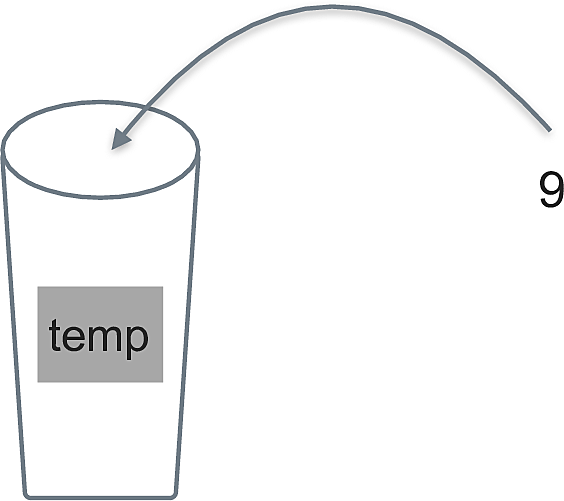
\includegraphics[width=0.25\textwidth,height=\textheight]{img/Variablen_zuweisen.png}

}

\caption{\label{fig-var-zuweisen}Wir definieren eine Variable ``temp''
mit dem Inhalt ``9''}

\end{figure}%

\subsection{Beobachtungseinheit}\label{beobachtungseinheit}

\begin{definition}[Beobachtungseinheit]\protect\hypertarget{def-beobeinheit}{}\label{def-beobeinheit}

Beobachtungseinheiten sind die Dinge, die wir untersuchen (beobachten).
Beobachtungseinheiten sind die Träger von Variablen.\(\square\)

\end{definition}

In Tabelle~\ref{tbl-daten} gibt es drei Variablen: \texttt{id},
\texttt{Name} und \texttt{Note}. Es gibt auch drei
Beobachtungseinheiten: \emph{Anna}, \emph{Berta} und \emph{Carla.}

\subsection{Wert}\label{wert}

\begin{definition}[]\protect\hypertarget{def-wert}{}\label{def-wert}

Ein \emph{Wert} ist der Inhalt einer Variablen.\(\square\)

\end{definition}

In Abbildung~\ref{fig-var-zuweisen} ist der Wert von \texttt{temp} 9. In
Tabelle~\ref{tbl-daten} hat die Variable \texttt{name} drei Elemente:
Anna, Berta, Carla. Der Wert des 2. Elements ist Berta.

\begin{definition}[]\protect\hypertarget{def-auspraegung}{}\label{def-auspraegung}

Als \emph{Ausprägungen} bezeichnet man die verschiedenen Werte einer
Variablen. \(\square\)

\end{definition}

\begin{example}[]\protect\hypertarget{exm-geschlecht}{}\label{exm-geschlecht}

In einer Studie wurden zehn Probanden untersucht. Die Variable
\texttt{geschlecht} dokumentiert die Geschlechter der Personen:

\begin{Shaded}
\begin{Highlighting}[]
\NormalTok{geschlecht }\OtherTok{\textless{}{-}} \FunctionTok{c}\NormalTok{(}\StringTok{"Mann"}\NormalTok{, }\StringTok{"Frau"}\NormalTok{, }\StringTok{"Frau"}\NormalTok{, }\StringTok{"Frau"}\NormalTok{, }\StringTok{"Mann"}\NormalTok{,}
                \StringTok{"Frau"}\NormalTok{, }\StringTok{"Mann"}\NormalTok{, }\StringTok{"Mann"}\NormalTok{, }\StringTok{"divers"}\NormalTok{, }\StringTok{"Frau"}\NormalTok{)}
\NormalTok{geschlecht}
\DocumentationTok{\#\#  [1] "Mann"   "Frau"   "Frau"   "Frau"   "Mann"   "Frau"   "Mann"   "Mann"  }
\DocumentationTok{\#\#  [9] "divers" "Frau"}
\end{Highlighting}
\end{Shaded}

In dieser Variable (die aus 10 Werten besteht) finden sich drei
Ausprägungen: divers, Frau, Mann.\(\square\)

\end{example}

\begin{tcolorbox}[enhanced jigsaw, toptitle=1mm, rightrule=.15mm, colbacktitle=quarto-callout-tip-color!10!white, breakable, title=\textcolor{quarto-callout-tip-color}{\faLightbulb}\hspace{0.5em}{Tipp}, bottomrule=.15mm, colback=white, opacitybacktitle=0.6, left=2mm, titlerule=0mm, toprule=.15mm, coltitle=black, opacityback=0, bottomtitle=1mm, arc=.35mm, leftrule=.75mm, colframe=quarto-callout-tip-color-frame]

Gerade haben Sie etwas Computer-Syntax gesehen, genauer gesagt, Befehle
aus der Programmiersprache \emph{R}. Bisher haben wir diese Befehle
nicht kennengelernt. Sie verstehen Sie vermutlich (nicht ganz).
Ignorieren Sie diese Befehle einfach erstmal.

\end{tcolorbox}

\subsection{Tidy-Data}\label{tidy-data}

\begin{definition}[]\protect\hypertarget{def-tidy}{}\label{def-tidy}

Unter \emph{Tidy-Data} (tidy data, ``Normalform'') versteht man eine
Tabelle, in der jede Zeile eine Beobachtungseinheit darstellt, jede
Spalte eine Variable und jede Zelle der Tabelle einen Wert, s.
Abbildung~\ref{fig-tidy1}. (Zusätzlich ist noch eine ``Kopfzeile''
erlaubt, in der die Namen der Variablen stehen.)\(\square\)

\end{definition}

Tabelle~\ref{tbl-daten} ist ein Beispiel für Tidy-Data.
Abbildung~\ref{fig-tidy1} zeigt ein Sinnbild für Tidy-Data (Wickham \&
Grolemund, 2018). Und Abbildung~\ref{fig-tidy-hadley} erläutert das
Tidy-Prinzip genauer.

\begin{figure}

\begin{minipage}{0.50\linewidth}

\centering{

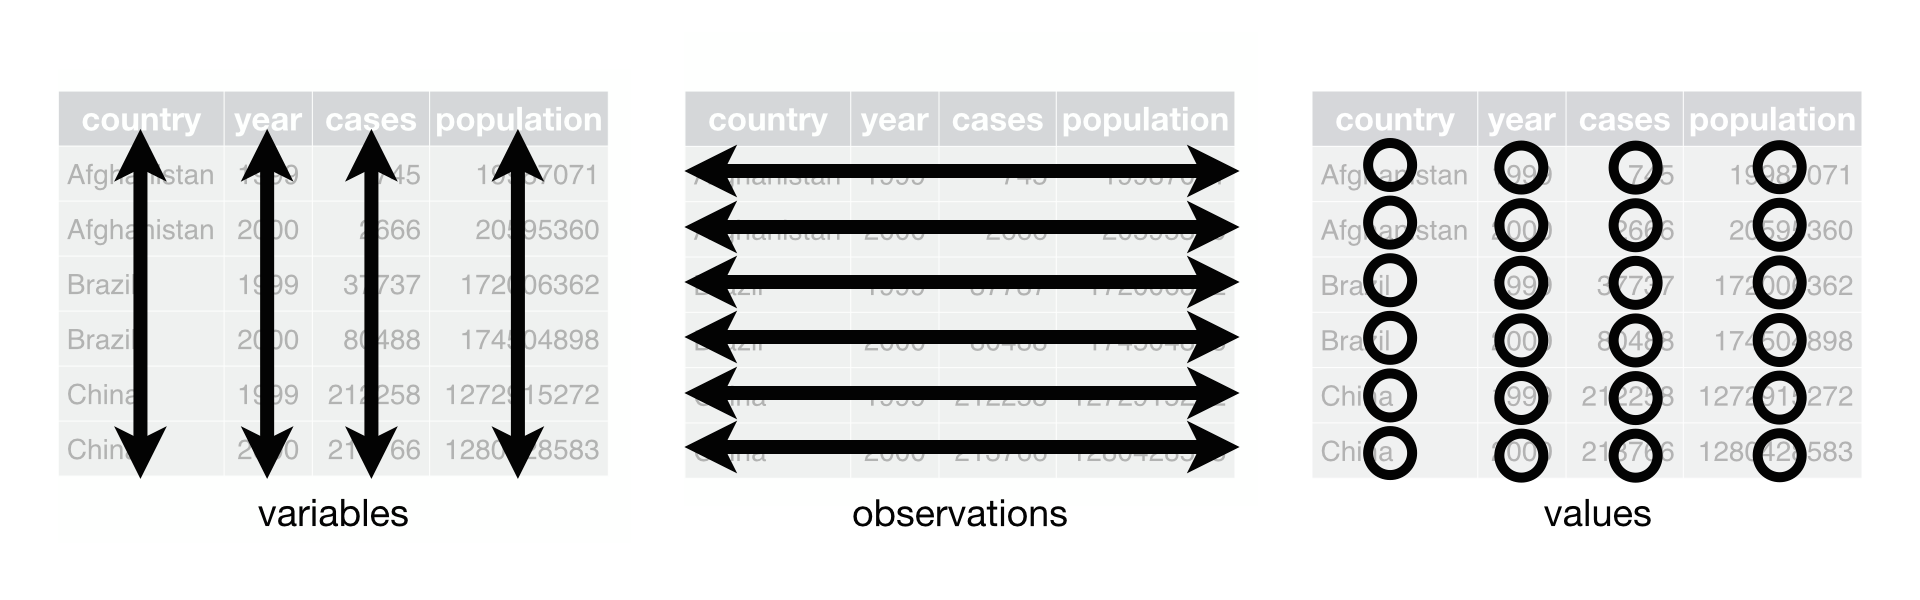
\includegraphics{img/tidy-1.png}

}

\subcaption{\label{fig-tidy1}Tidy-Data-Sinnbild. Image Credit: Hadley
Wickham}

\end{minipage}%
%
\begin{minipage}{0.50\linewidth}

\centering{

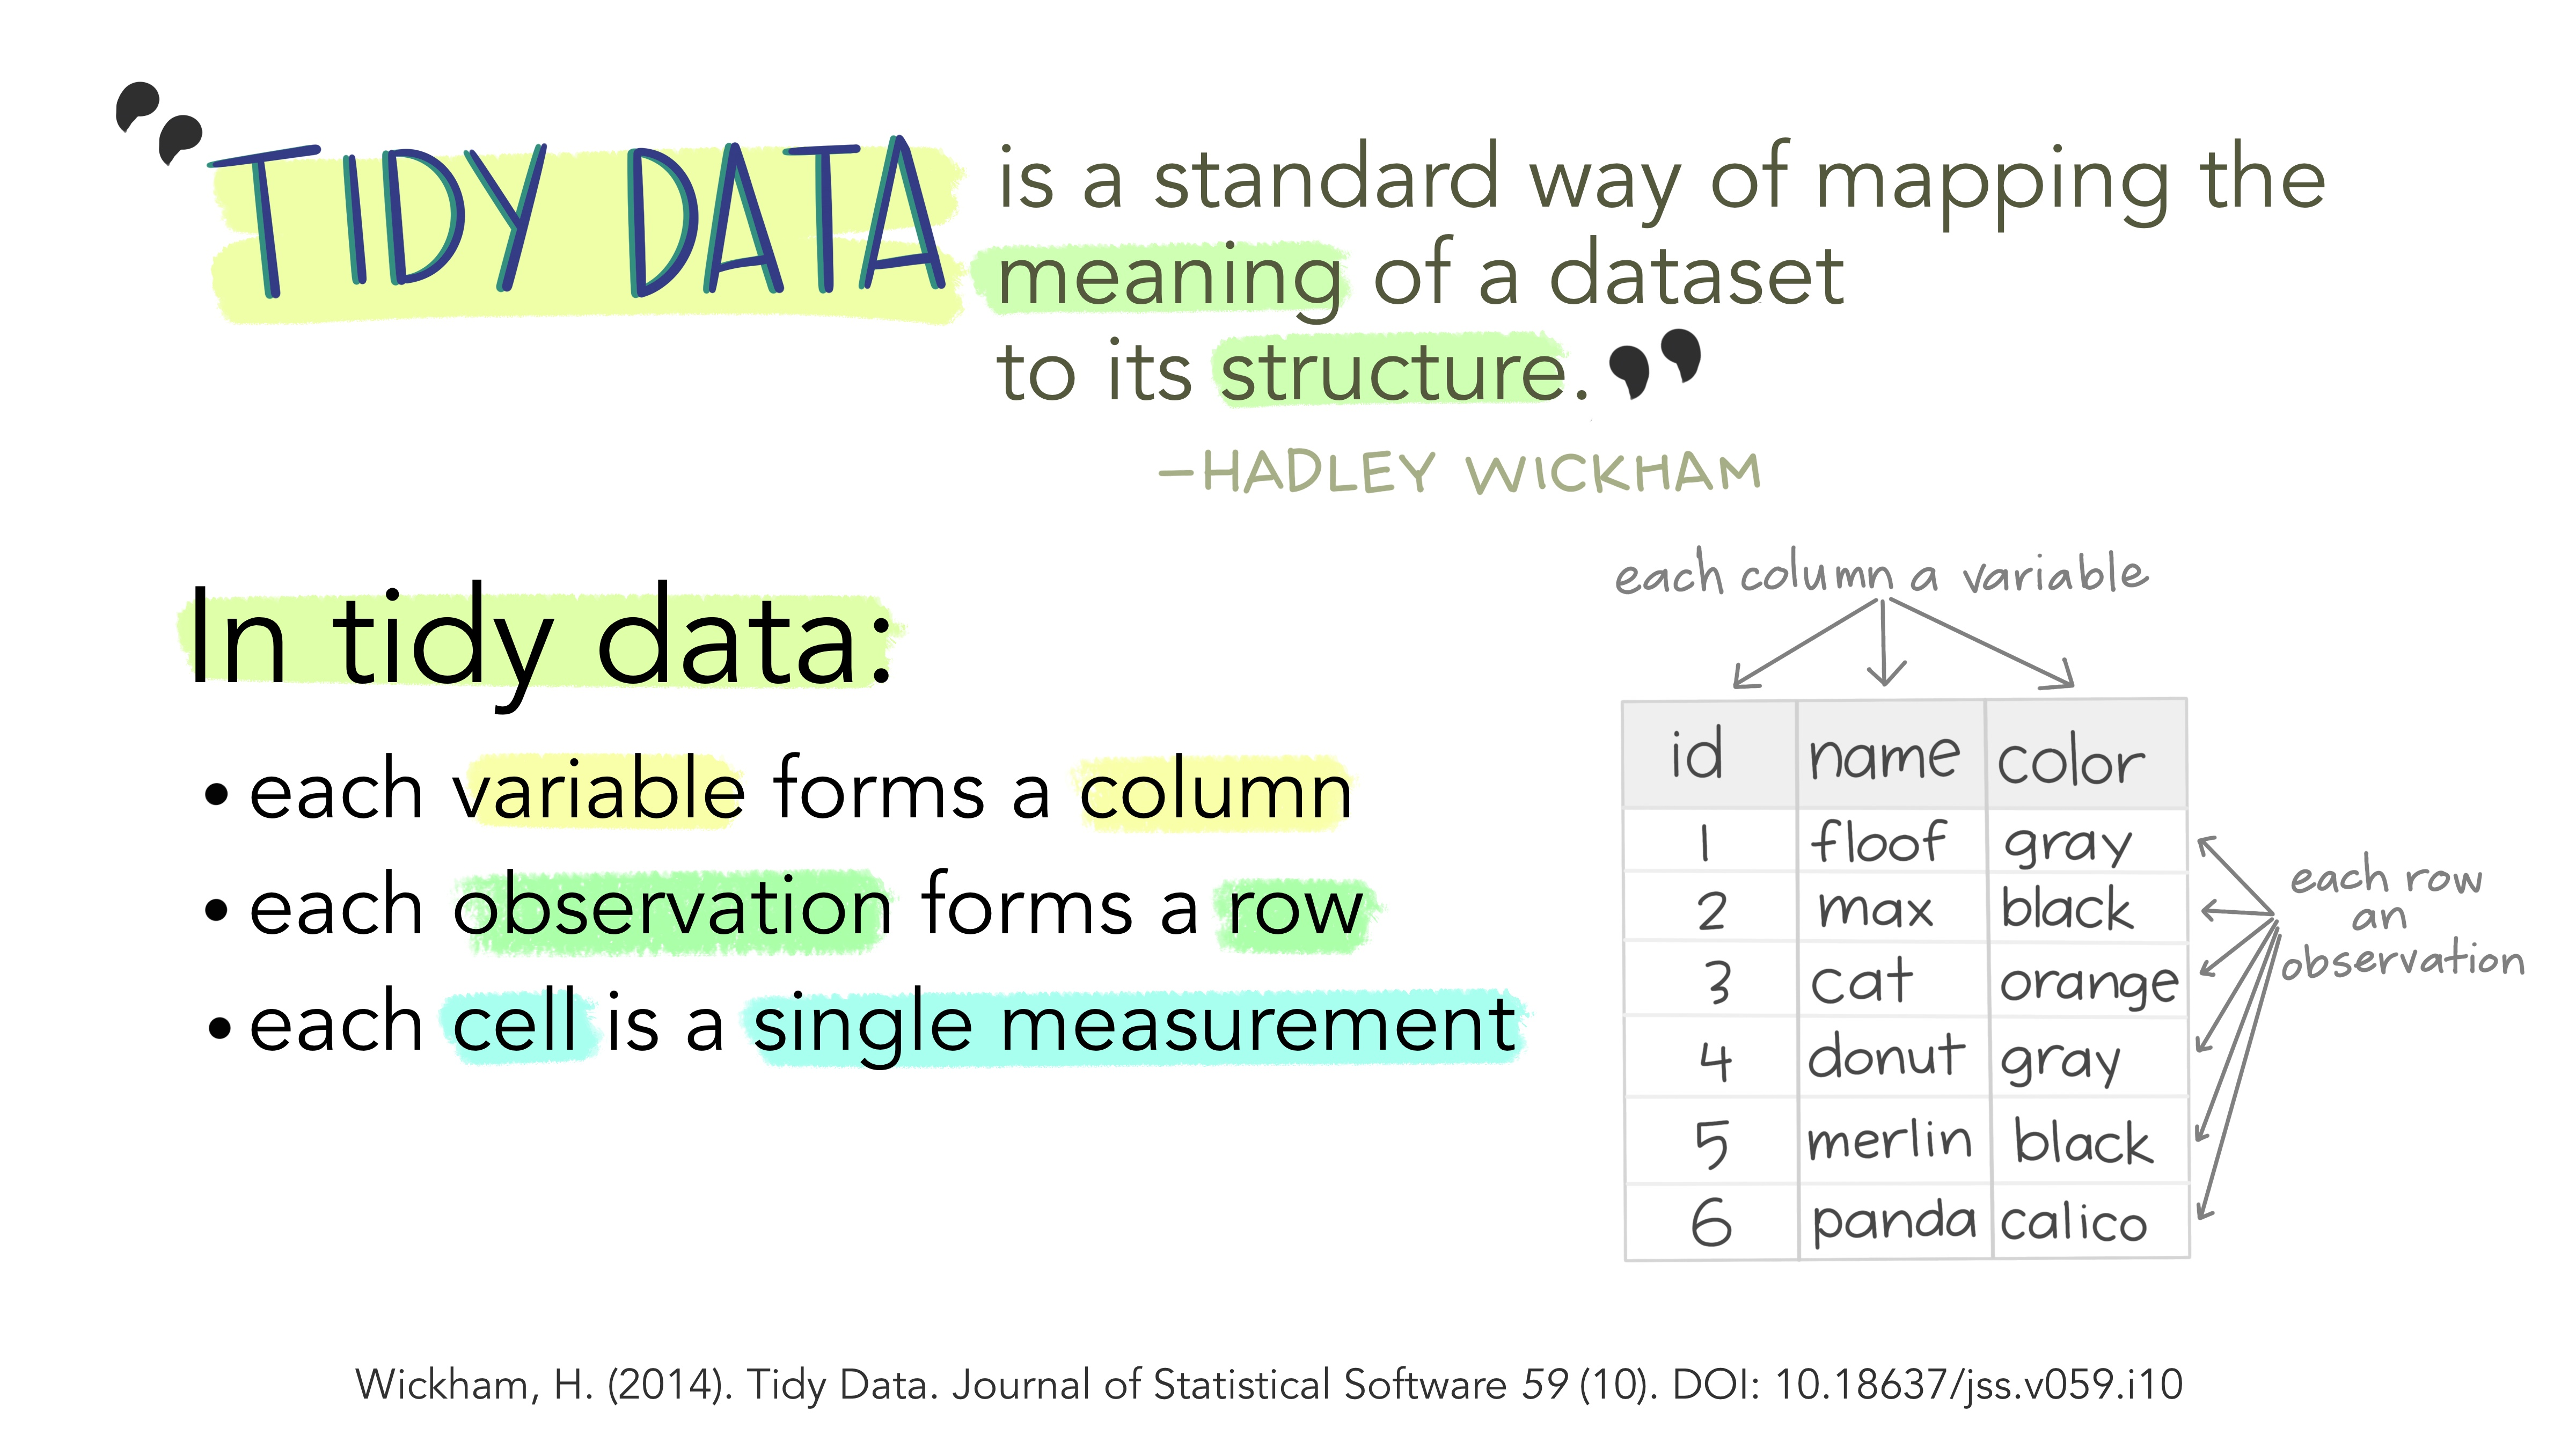
\includegraphics{img/tidydata_1.jpg}

}

\subcaption{\label{fig-tidy-hadley}Was ist Tidy-Data?. Image Credit:
Allision Horst}

\end{minipage}%

\caption{\label{fig-tidy-all}Stay Tidy!}

\end{figure}%

\begin{tcolorbox}[enhanced jigsaw, toptitle=1mm, rightrule=.15mm, colbacktitle=quarto-callout-important-color!10!white, breakable, title=\textcolor{quarto-callout-important-color}{\faExclamation}\hspace{0.5em}{Wichtig}, bottomrule=.15mm, colback=white, opacitybacktitle=0.6, left=2mm, titlerule=0mm, toprule=.15mm, coltitle=black, opacityback=0, bottomtitle=1mm, arc=.35mm, leftrule=.75mm, colframe=quarto-callout-important-color-frame]

Für eine statistische Analyse ist es oft sinnvoll, dass die Daten im
Tidy-Format vorliegen.

\end{tcolorbox}

Der Vorteil des Tidy-Formats ist es, dass man weiß, wie die Daten
aufgebaut sind. Außerdem können Statistikprogramme oft mit dieser Form
am besten umgehen, s. fig-tidy3.

\begin{figure}

\centering{

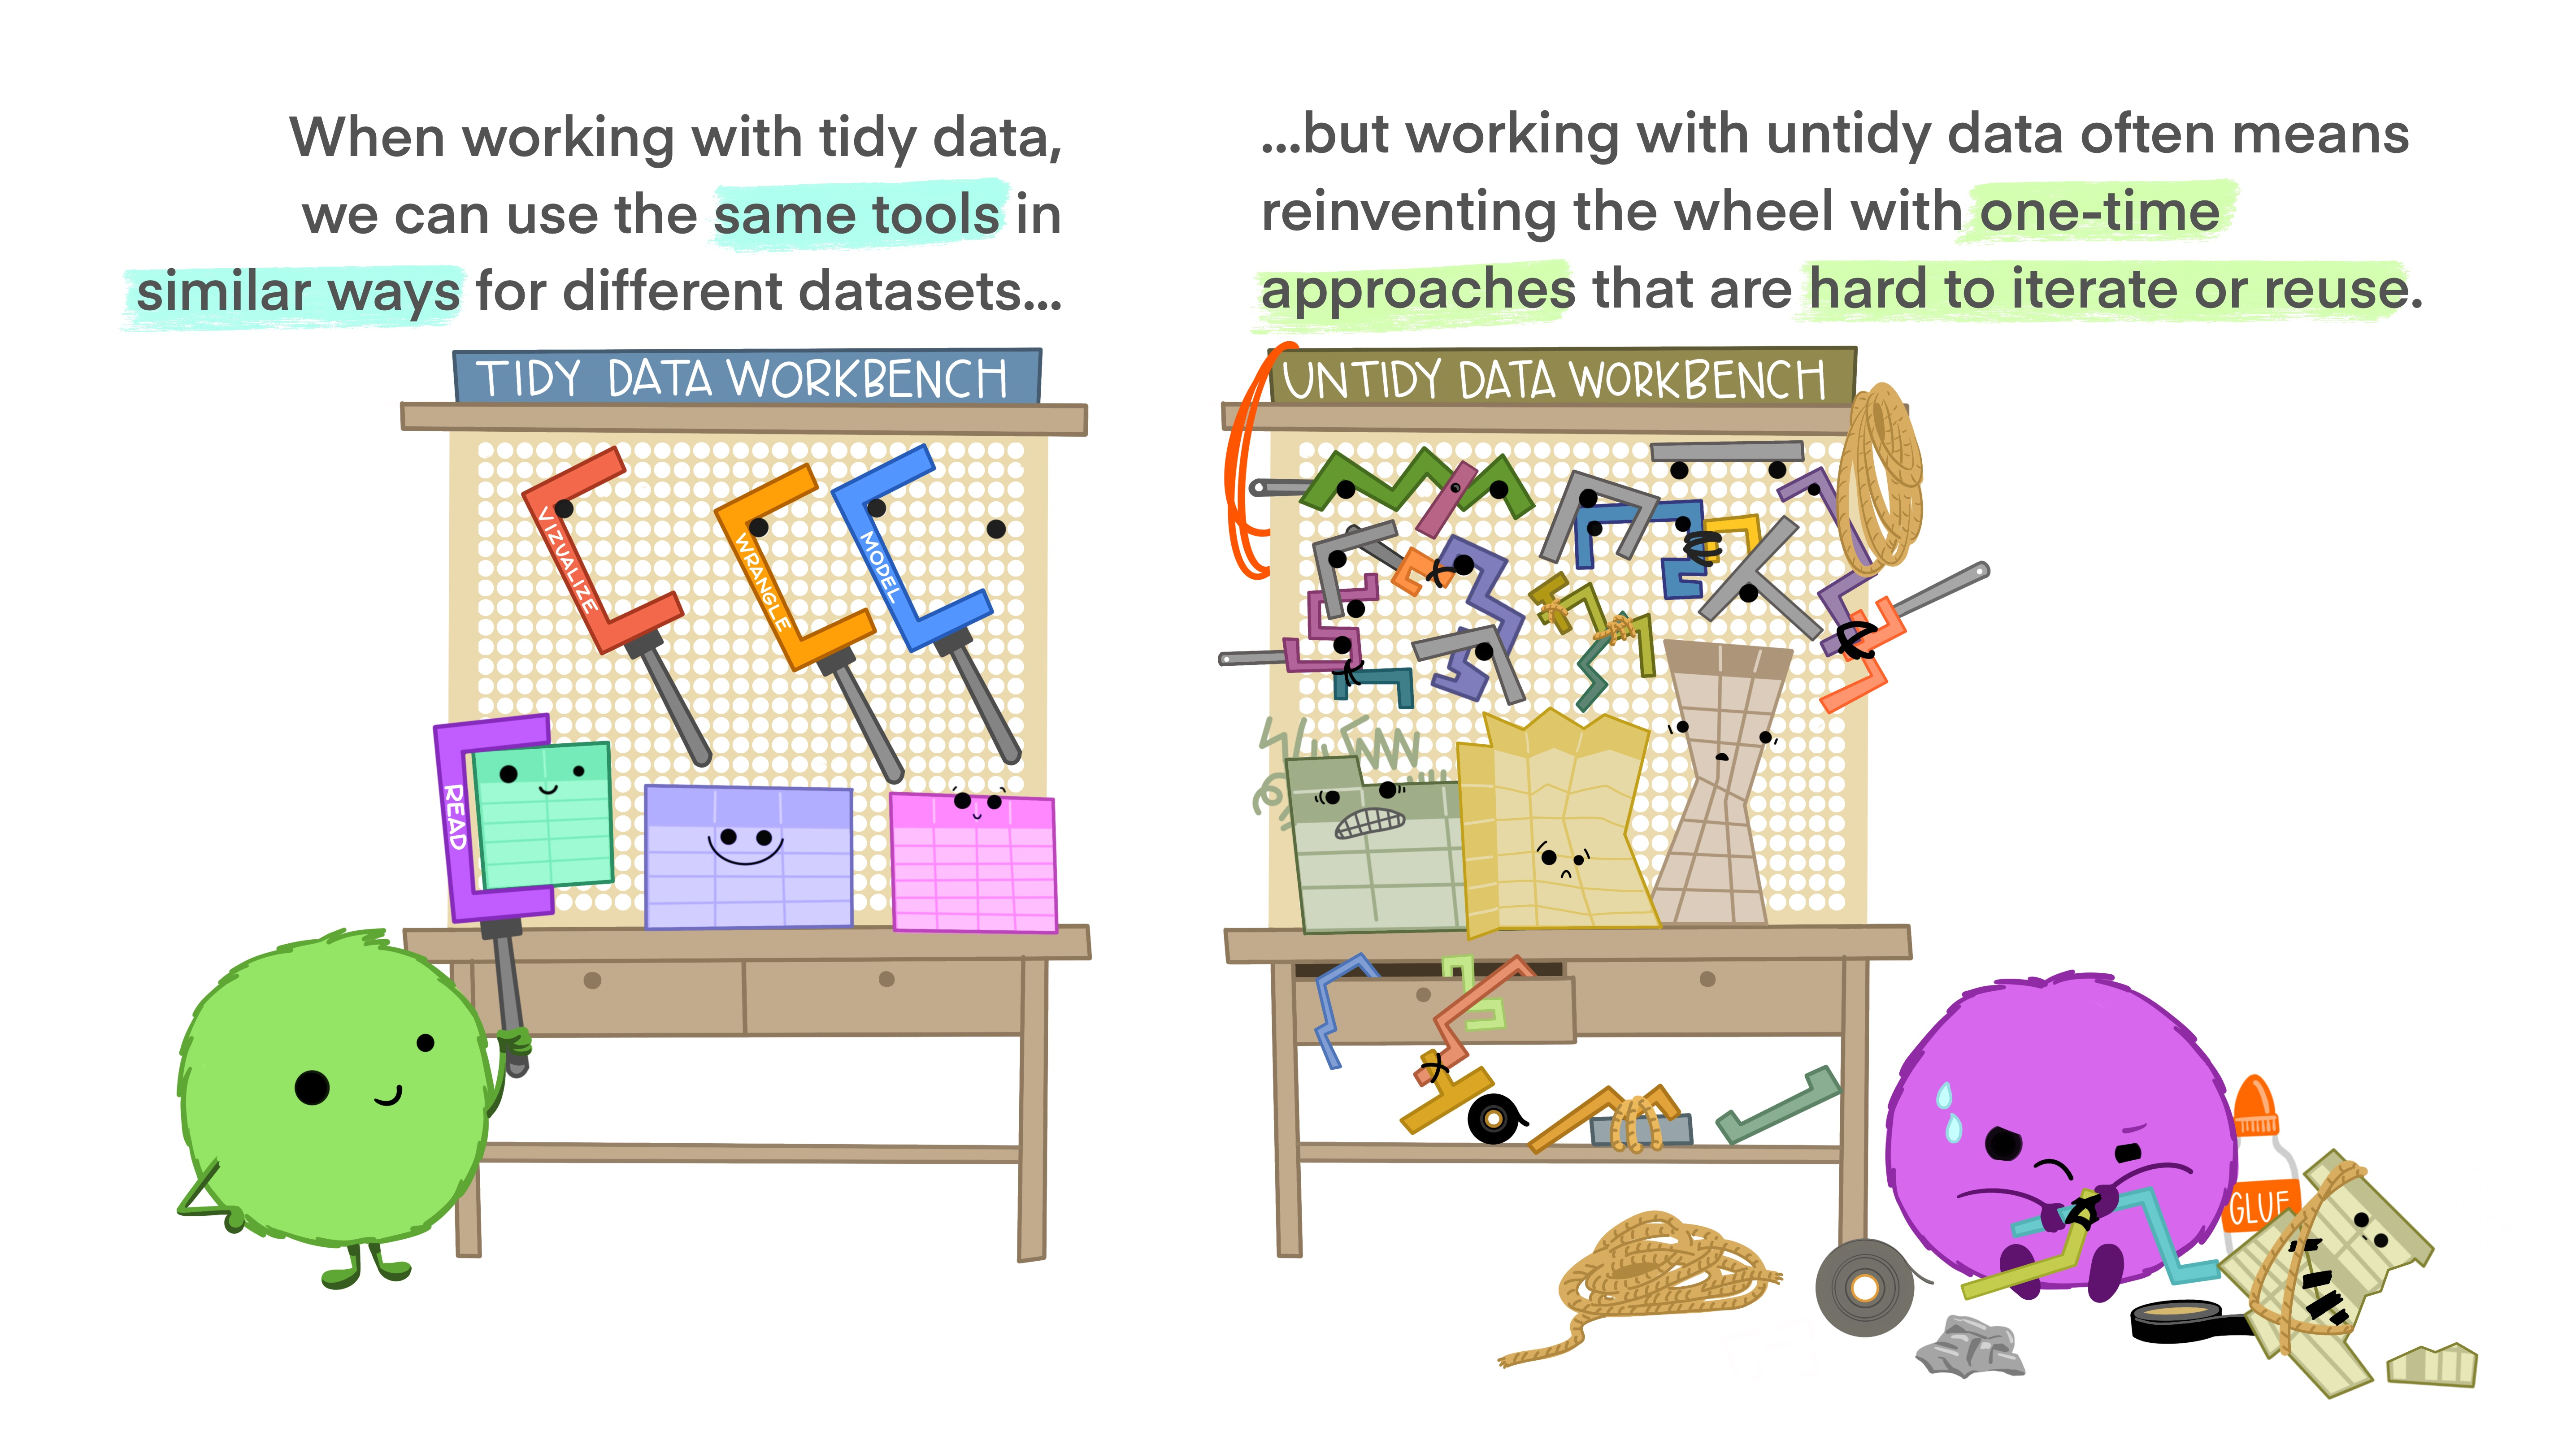
\includegraphics[width=0.5\textwidth,height=\textheight]{img/tidydata_3.jpg}

}

\caption{\label{fig-tidy3}Immer schön Ordnung halten\ldots{} Image
credit: Allision Horst}

\end{figure}%

\href{https://github.com/allisonhorst/stats-illustrations}{Quelle}

Das Tidy-Format wird auch als ``langes'' Format bezeichnet.

Abbildung~\ref{fig-long-wide-anim} zeigt einen Datensatz in der
``langen'' Form, also tidy, und den gleichen Datensatz, umformatiert in
der ``breiten'' Form, nicht-tidy.

\begin{figure}

\centering{

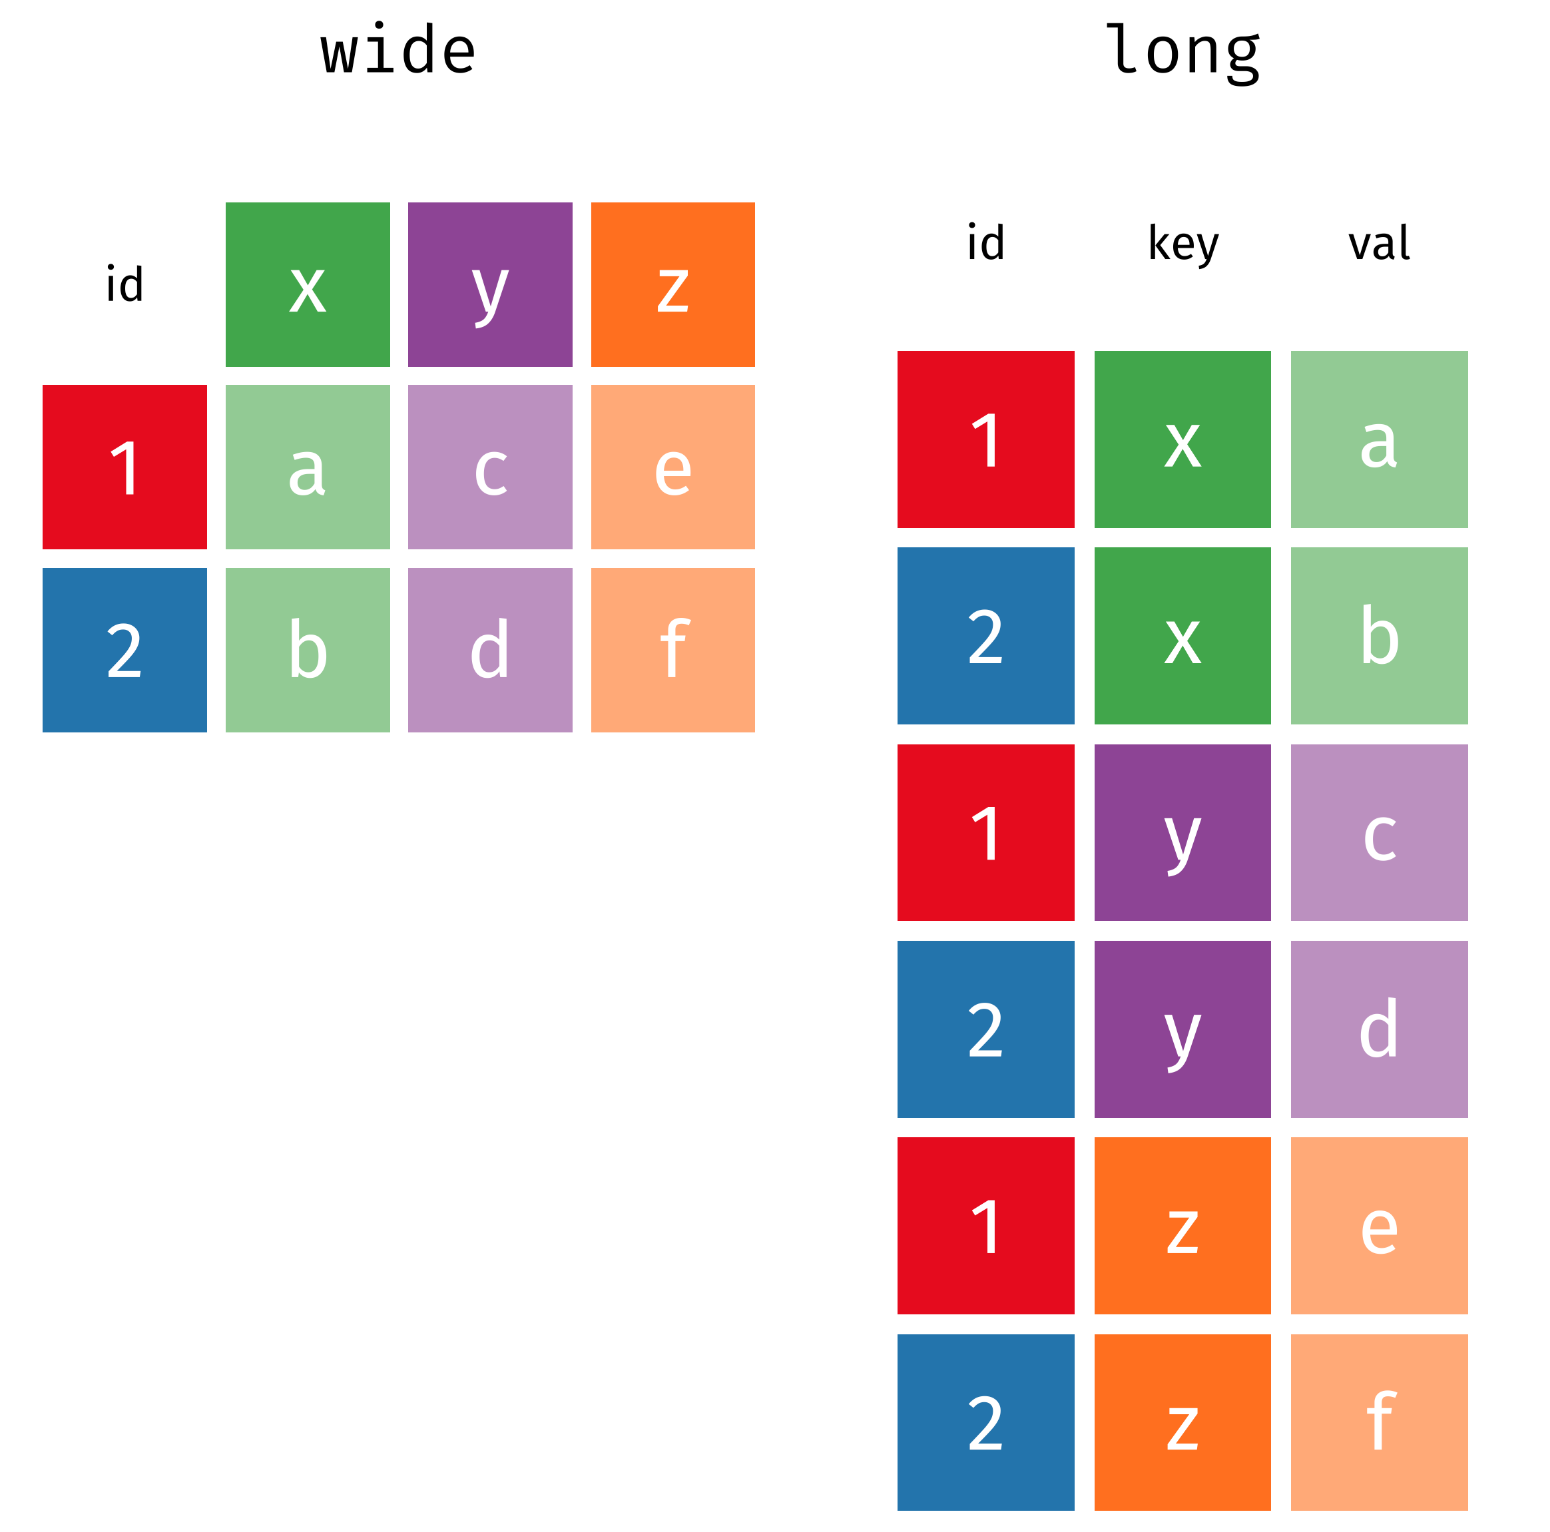
\includegraphics[width=0.5\textwidth,height=\textheight]{img/wide-long.png}

}

\caption{\label{fig-long-wide-anim}Links: Eine Tabelle mit Format
``wide'' - nicht ``tidy''. Rechts: Das ``Langformat'' (``long'') ist
``tidy''.}

\end{figure}%

{Quelle: Garrick Aden-Buie, 2018, CC0-1.0 license,
https://www.garrickadenbuie.com/project/tidyexplain/}

\begin{tcolorbox}[enhanced jigsaw, toptitle=1mm, rightrule=.15mm, colbacktitle=quarto-callout-tip-color!10!white, breakable, title=\textcolor{quarto-callout-tip-color}{\faLightbulb}\hspace{0.5em}{Tipp}, bottomrule=.15mm, colback=white, opacitybacktitle=0.6, left=2mm, titlerule=0mm, toprule=.15mm, coltitle=black, opacityback=0, bottomtitle=1mm, arc=.35mm, leftrule=.75mm, colframe=quarto-callout-tip-color-frame]

In vielen Organisationen werden Exceltabellen für bestimmte Zwecke der
Datenverarbeitung verwendet. Excel\footnotemark{} hat bestimmte Stärken
und Vorteile, aber auch gewisse Nachteile und Schwäche; das liegt z.T.
daran, dass Excel für bestimmte Aufgaben besser und für andere weniger
gut geeignet ist. Wenn man mit Excel arbeitet, wiederholen sich
erfahrungsgemäß immer wieder die gleichen Fehler bzw. suboptimalen
Vorgehensweise zum Aufbau einer Exceltabelle.

\href{https://www.tandfonline.com/doi/full/10.1080/00031305.2017.1375989}{Dieser
Artikel} von Broman \& Woo (2018) zeigt anhand einiger praktischer
Tipps, wie man Exceltabellen so aufbaut, dass Fehler minimiert werden.

\end{tcolorbox}

\footnotetext{und ähnliche Programme}

\section{Arten von Variablen}\label{sec-arten-variablen}

\subsection{Nach Position in der
Forschungsfrage}\label{nach-position-in-der-forschungsfrage}

Angenommen, Ihre Forschungsfrage lautet:

\begin{quote}
Hat Lernen einen Einfluss auf den Prüfungserfolg?
\end{quote}

In dem Fall gilt:

\begin{itemize}
\tightlist
\item
  \emph{Lernen} ist die Inputvariable/X-Variable/Ursache/unabhängig
  Variable (UV)
\item
  \emph{Prüfungserfolg} ist die
  Outputvariable/Y-Variable/Wirkung/abhängige Variable (AV)
\end{itemize}

Abbildung~\ref{fig-ueberblick-fragen} stellt diese beiden ``Positionen''
einer Variable dar. Die erste Position ist vor dem Pfeil. Die zweite
Position ist nach dem Pfeil.

\begin{figure}

\centering{

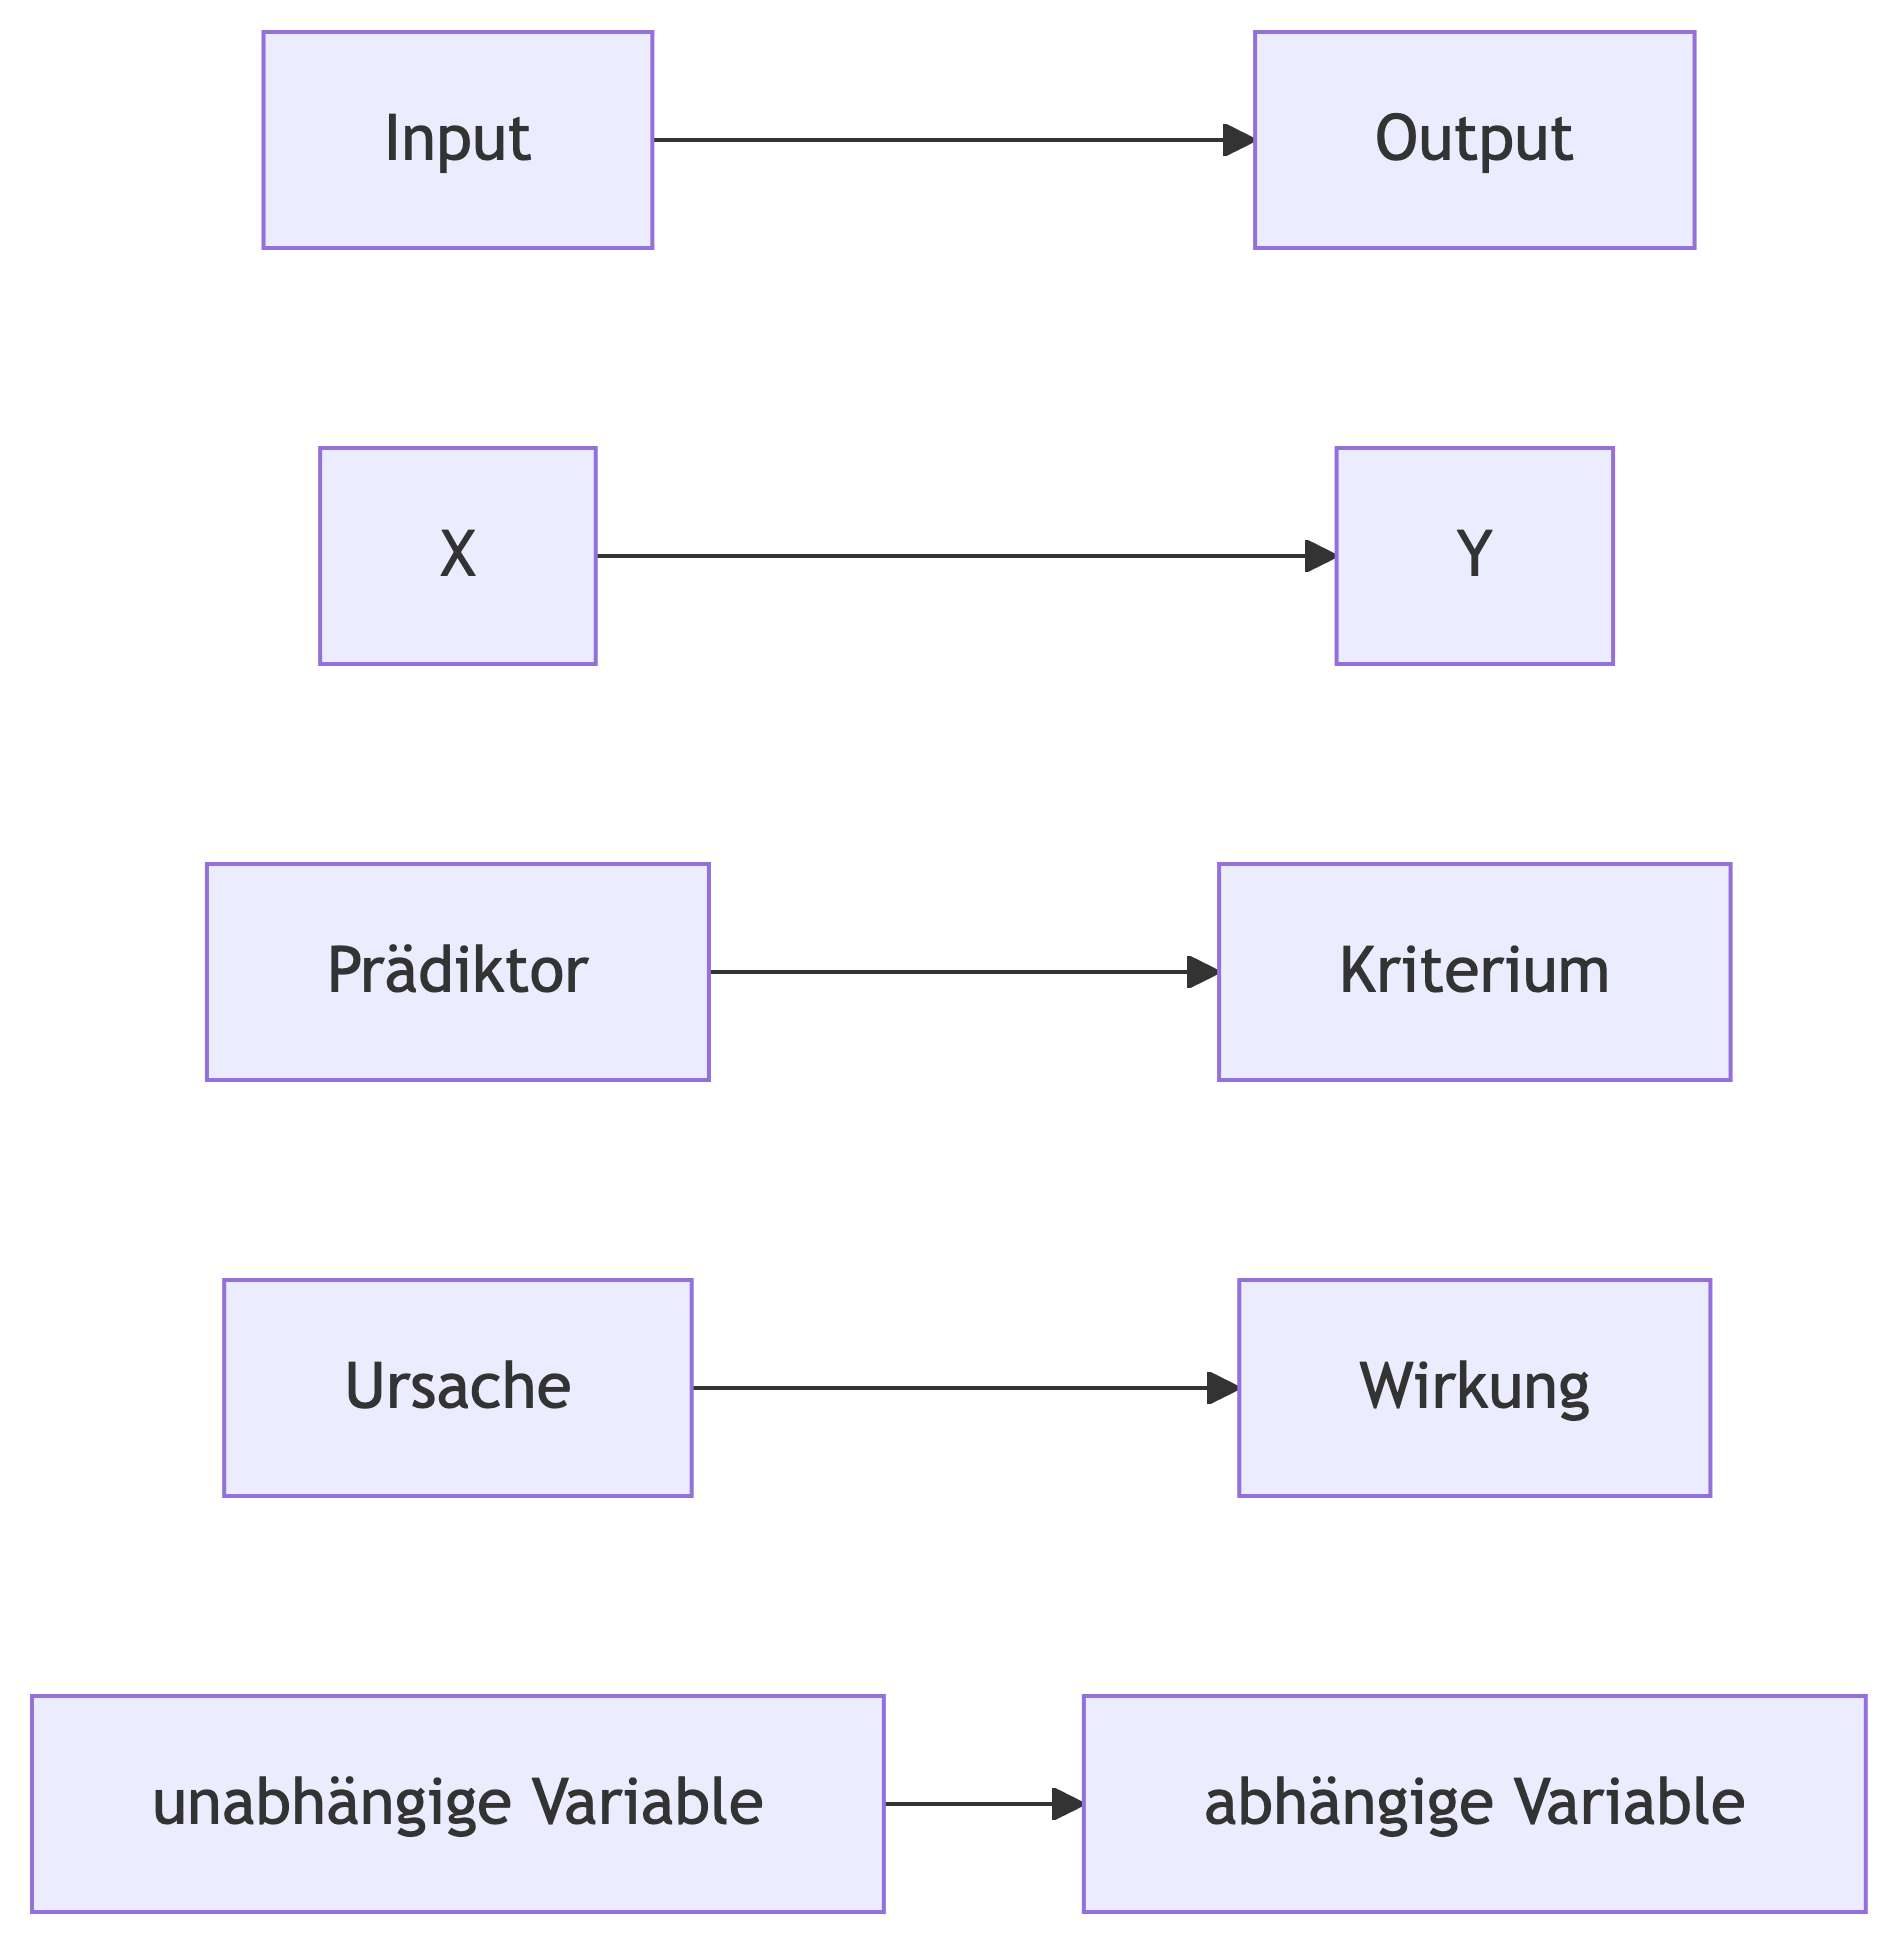
\includegraphics[width=4in,height=3.99in]{010-rahmen_files/figure-latex/mermaid-figure-3.png}

}

\caption{\label{fig-ueberblick-fragen}Synonyme Bezeichnungen für Input-
und Output-Variablen einer Forschungsfrage}

\end{figure}%

\begin{exercise}[]\protect\hypertarget{exr-uvav}{}\label{exr-uvav}

Überlegen Sie sich eine Forschungsfrage, die eine UV und eine AV
enthält. Sagen Sie einer/em Kommilitonen diese Forschungsfrage und
fragen Sie, was die UV und die AV ist. Bei richtiger Antwort belohnen
Sie großzügig. \(\square\)

\end{exercise}

\subsection{Nach dem Skalenniveau}\label{nach-dem-skalenniveau}

\begin{definition}[]\protect\hypertarget{def-skalenniveau}{}\label{def-skalenniveau}

Der Begriff \emph{Skalenniveau} wird verwendet, um die Art und Menge der
Information, die in Variablen enthalten ist, zu benennen. Diese
Klassifikation basiert auf den Eigenschaften der Daten und den
mathematischen Operationen, die sinnvoll auf diese Daten angewendet
werden können. \(\square\)

\end{definition}

Abbildung~\ref{fig-skalenniveau} gibt einen Überblick über typisch
verwendete Skalenniveaus.

\begin{figure}

\centering{

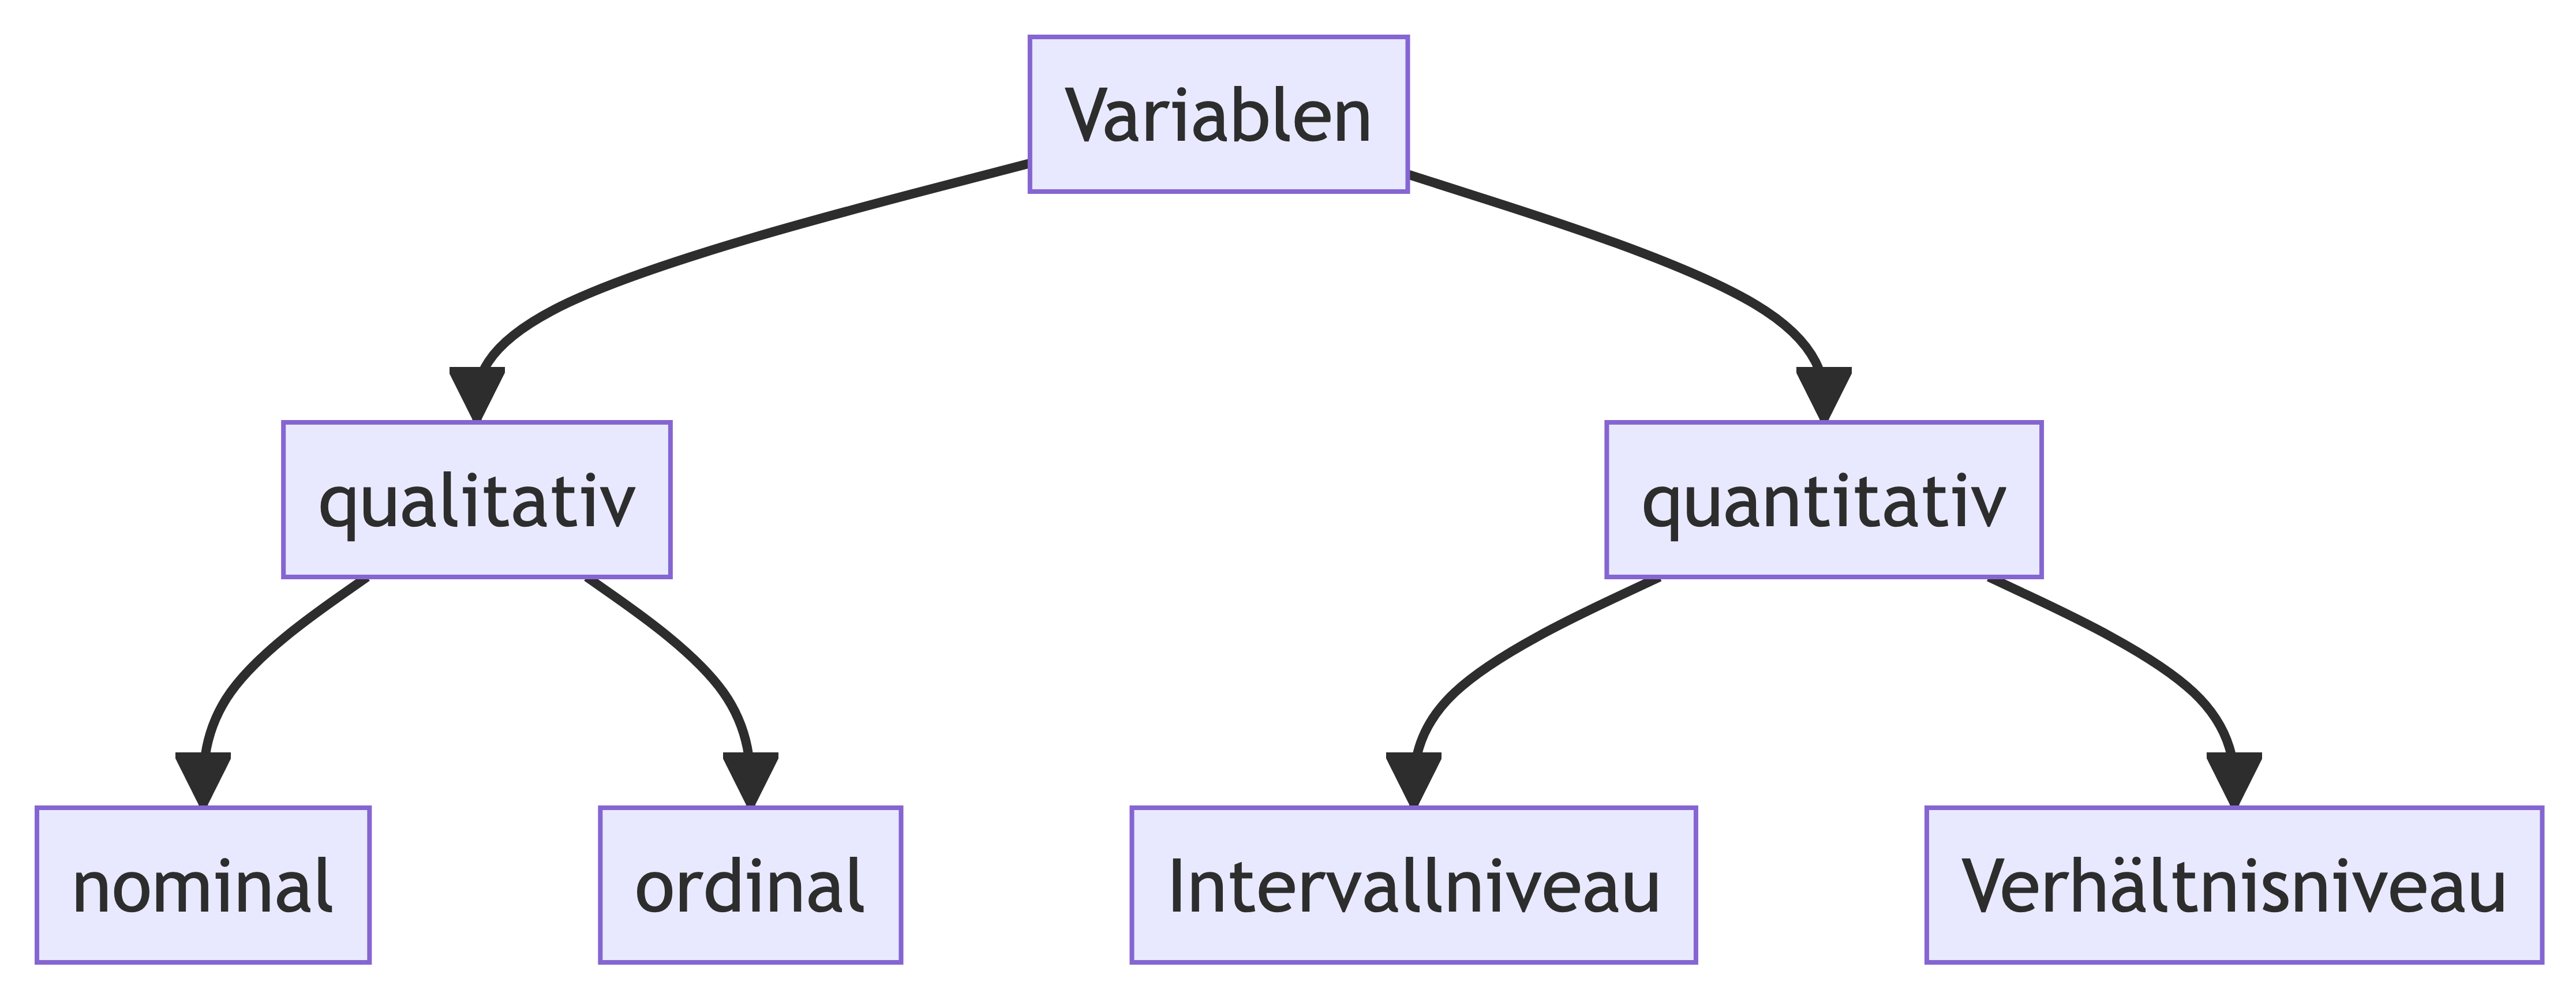
\includegraphics[width=5.82in,height=2.26in]{010-rahmen_files/figure-latex/mermaid-figure-2.png}

}

\caption{\label{fig-skalenniveau}Skalenniveaus}

\end{figure}%

\subsection{Beispiele für
Skalenniveaus}\label{beispiele-fuxfcr-skalenniveaus}

Beispiele zu den Skalenniveaus sind in Tabelle~\ref{tbl-skalen-bsps}
aufgeführt. \(\square\)

\begin{longtable}[]{@{}ll@{}}

\caption{\label{tbl-skalen-bsps}Beispiele für Skalenniveaus}

\tabularnewline

\toprule\noalign{}
Variable & Skalenniveau \\
\midrule\noalign{}
\endhead
\bottomrule\noalign{}
\endlastfoot
Haarfarbe & Nominalskala \\
Augenfarbe & Nominalskala \\
Geschlecht & Nominalskala \\
Automarke & Nominalskala \\
Partei & Nominalskala \\
Lieblingsessen & Ordinalskala \\
Medaillen beim 100-Meter-Lauf & Ordinalskala \\
Uniranking & Ordinalskala \\
IQ & Intervallskala \\
Extraversion & Intervallskala \\
Temperatur in Celcius & Intervallskala \\
Temperatur in Fahrenheit & Intervallskala \\
Temperatur in Kelvin & Verhältnisskala \\
Körpergröße & Verhältnisskala \\
Geschwindigkeit & Verhältnisskala \\
Länge & Verhältnisskala \\

\end{longtable}

Je nach dem, über welches Skalenniveau eine Variable verfügt, sind
verschiedenen Rechenoperationen erlaubt, s. {tbl-skalenniveaus-pdf}.

\begin{longtable}[]{@{}
  >{\raggedright\arraybackslash}p{(\columnwidth - 10\tabcolsep) * \real{0.2237}}
  >{\raggedright\arraybackslash}p{(\columnwidth - 10\tabcolsep) * \real{0.1579}}
  >{\raggedright\arraybackslash}p{(\columnwidth - 10\tabcolsep) * \real{0.1447}}
  >{\raggedright\arraybackslash}p{(\columnwidth - 10\tabcolsep) * \real{0.1579}}
  >{\raggedright\arraybackslash}p{(\columnwidth - 10\tabcolsep) * \real{0.1184}}
  >{\raggedright\arraybackslash}p{(\columnwidth - 10\tabcolsep) * \real{0.1974}}@{}}

\caption{\label{tbl-skalenniveaus-pdf}Erlaubte Rechenoperationen nach
Skalenniveau}

\tabularnewline

\toprule\noalign{}
\begin{minipage}[b]{\linewidth}\raggedright
Skalenniveau
\end{minipage} & \begin{minipage}[b]{\linewidth}\raggedright
Quantitativ
\end{minipage} & \begin{minipage}[b]{\linewidth}\raggedright
Gleichheit
\end{minipage} & \begin{minipage}[b]{\linewidth}\raggedright
Reihenfolge
\end{minipage} & \begin{minipage}[b]{\linewidth}\raggedright
Addition
\end{minipage} & \begin{minipage}[b]{\linewidth}\raggedright
Multiplikation
\end{minipage} \\
\midrule\noalign{}
\endhead
\bottomrule\noalign{}
\endlastfoot
Nominalniveau & nein & ja & nein & nein & nein \\
Ordinalniveau & nein & ja & ja & nein & nein \\
Intervallniveau & ja & ja & ja & ja & nein \\
Verhältnisniveau & ja & ja & ja & ja & ja \\

\end{longtable}

Was soll das bedeuten, ``Rechenoperationen''?

Schauen wir uns für jedes Skalenniveau ein ``Rechenbeispiel'' an.

\emph{Nominalskala}: Die Variable \emph{Geschlecht} ist nominalskaliert.
Das bedeutet, dass ihre Ausprägungen \emph{Frau} und \emph{Mann} z.B.
nicht (sinnvoll) addiert oder sonstwie ``verrechnet'' werden können. Man
könnte, z.B. um das Eintippen zu erleichtern, Frauen mit \texttt{1}
kodieren und Männer mit \texttt{2}. Damit darf man aber nicht rechnen!
Nicht addieren, multiplizieren \ldots{} Es macht keinen Sinn zu sagen:
``Ich habe eine Frau und einen Mann in meiner Tabelle, das ist im
Schnitt ein diverses Geschlecht, weil der Mittelwert von 1 und 2 ist
1,5!''

Die \emph{einzige} ``Rechenoperation'', die man auf der Nominalskala
machen darf, ist die Prüfung auf \emph{Gleichheit}: Mann kann
feststellen, ob ein Objekt gleich zu einem anderen ist oder
unterschiedlich. Also ob zwei Personen das gleiche Geschlecht haben oder
von unterschiedlichem Geschlecht sind. Anders ausgedrückt:

\begin{itemize}
\tightlist
\item
  FRAU \(\ne\) MANN
\item
  FRAU \(=\) FRAU
\item
  MANN \(=\) MANN
\end{itemize}

\emph{Ordinalskala}: Diese Skala entspricht einer Rangordnung. Eine
Rangordnung ist etwa die geordnete Abfolge Ihres
Leibgerichte\footnote{1. Pizza, 2. Spagetthi, 3. Schnitzel}. Etwas
``formaler'' ausgedrückt:

\begin{itemize}
\tightlist
\item
  \(\text{Pizza} \succ \text{Spagetthi} \succ \text{Schnitzel}\)
\end{itemize}

Das komische Zeichen \(\succ\) soll heißen: ``Ist auf meiner Liste von
Leibgerichten weiter oben, mag ich lieber''. Man kann aber \emph{nicht}
sagen, ``Ich mag aber Pizza um 42\% mehr als die Spagetthi und die
wieder um 73\% mehr als ein Schnitzel!''. Zumindest kann man das nicht
ohne weitere Informationen und Annahmen. Es gibt also Dinge auf der
Welt, die man leicht in eine Rangordnung bringen kann, aber die man nur
schwer in der Größe der Unterschiede bemessen kann. Das ist die
Ordinalskala.

\begin{tcolorbox}[enhanced jigsaw, toptitle=1mm, rightrule=.15mm, colbacktitle=quarto-callout-important-color!10!white, breakable, title=\textcolor{quarto-callout-important-color}{\faExclamation}\hspace{0.5em}{Wichtig}, bottomrule=.15mm, colback=white, opacitybacktitle=0.6, left=2mm, titlerule=0mm, toprule=.15mm, coltitle=black, opacityback=0, bottomtitle=1mm, arc=.35mm, leftrule=.75mm, colframe=quarto-callout-important-color-frame]

Die Ordinalskale erlaubt, Objekte zu ordnen (hinsichtlich eines
Merkmals). Die Abstände zwischen den Objekten können nicht quantifiziert
werden. \(\square\)

\end{tcolorbox}

\emph{Intervallskala}: Das ist vielleicht eine Überraschung für Sie:
Wenn es heute 10°C hat und morgen 5°C -- dann ist es heute \emph{nicht}
doppelt so warm wie morgen. Ja, 10 ist das Doppelte von 5. Aber
\emph{10° Celcius} ist \emph{nicht} doppelt so warm wie 20° Celcius.
Wenn Sie das verwundert: Das ist normal, so geht es vielen Leuten, wenn
sie das zum ersten Mal hören. Der Grund, dass es nicht erlaubt ist,
Verhältnisse (wie doppelt/halb so viel etc.) auf der Celcius-Skala zu
bilden, ist, dass der Nullpunkt der Skala, 0° C, kein echter,
physikalischer Nullpunkt ist. Bei 0° C liegt eben nicht Null
Wärmeenergie vor. Stattdessen wurde eine Wärmenergiemenge gewählt, die
für uns Menschen ganz praktisch, da augenfällig ist: der Gefrierpunkt
von Wasser. Was bei der Intervallskala erlaubt ist, ist das Addieren
(und Subtrahieren): heute 10°C, morgen 5°C, das ist ein Unterschied von
5°C. Oder: Im Schnitt waren es 7,5°C, das ist genau in der Mitte von 5
und 10°C. Abbildung~\ref{fig-intervall} versinnbildlicht die
Intervallskala.

\begin{figure}

\centering{

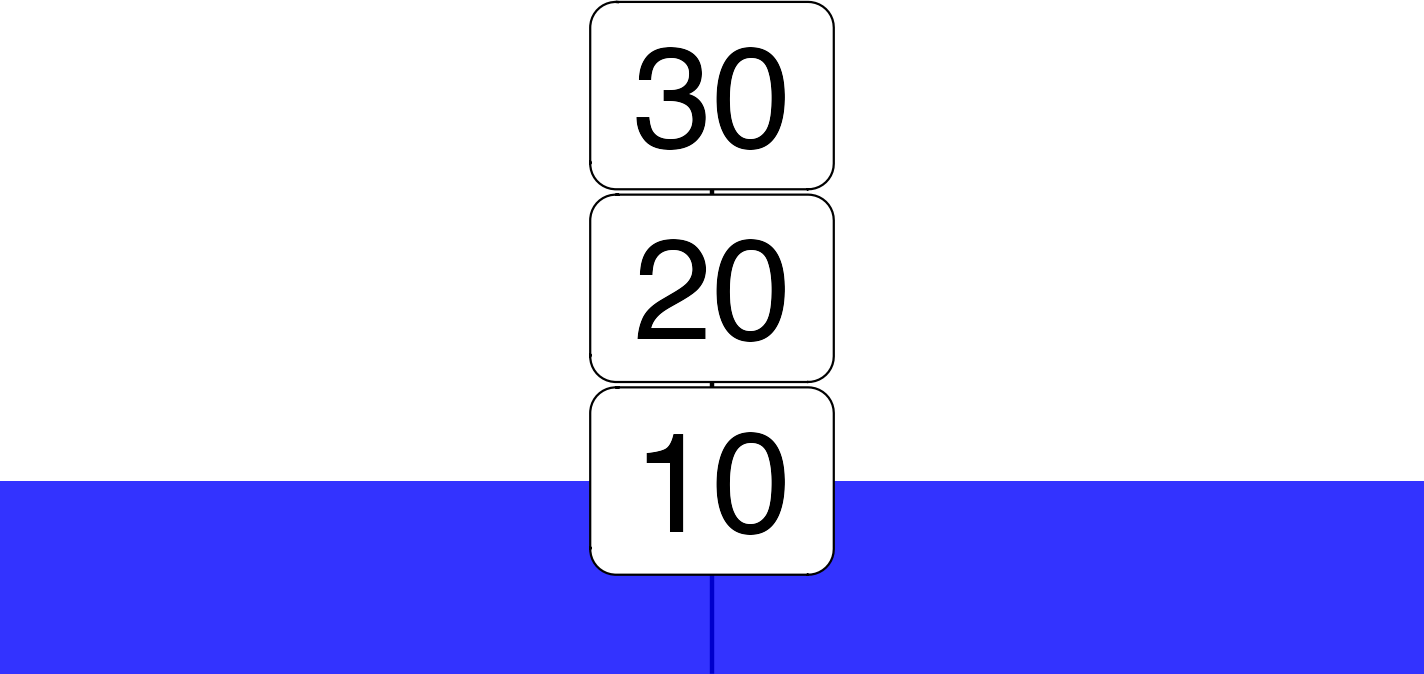
\includegraphics[width=1\textwidth,height=\textheight]{010-rahmen_files/figure-pdf/fig-intervall-1.png}

}

\caption{\label{fig-intervall}Ein Metermaß steckt im Wasser. Auf dem
Metermaß können wir die aufgedruckten Zahlen ablesen. Aber wir wissen
nicht, ob der Metermaß auf dem Boden steht. Wir wissen demnach nicht, ob
der vom Metermaß angegebene Nullpunkt der wahre Nullpunkt (Meeresboden)
ist.}

\end{figure}%

\emph{Verhältnisskala}: Eine Verhältnisskala ist das, was man sich
gemeinhin unter einer metrische Variable vorstellt: Man kann ``normal''
rechnen, alle Rechenoperationen sind erlaubt. Zuzüglich zu denen, die
auch in anderen, ``niedrigeren'' Skalenniveaus erlaubt sind, ist das das
Bilden von Verhältnissen - Multiplizieren, s.
Abbildung~\ref{fig-verhaeltnis}.

\begin{figure}

\centering{

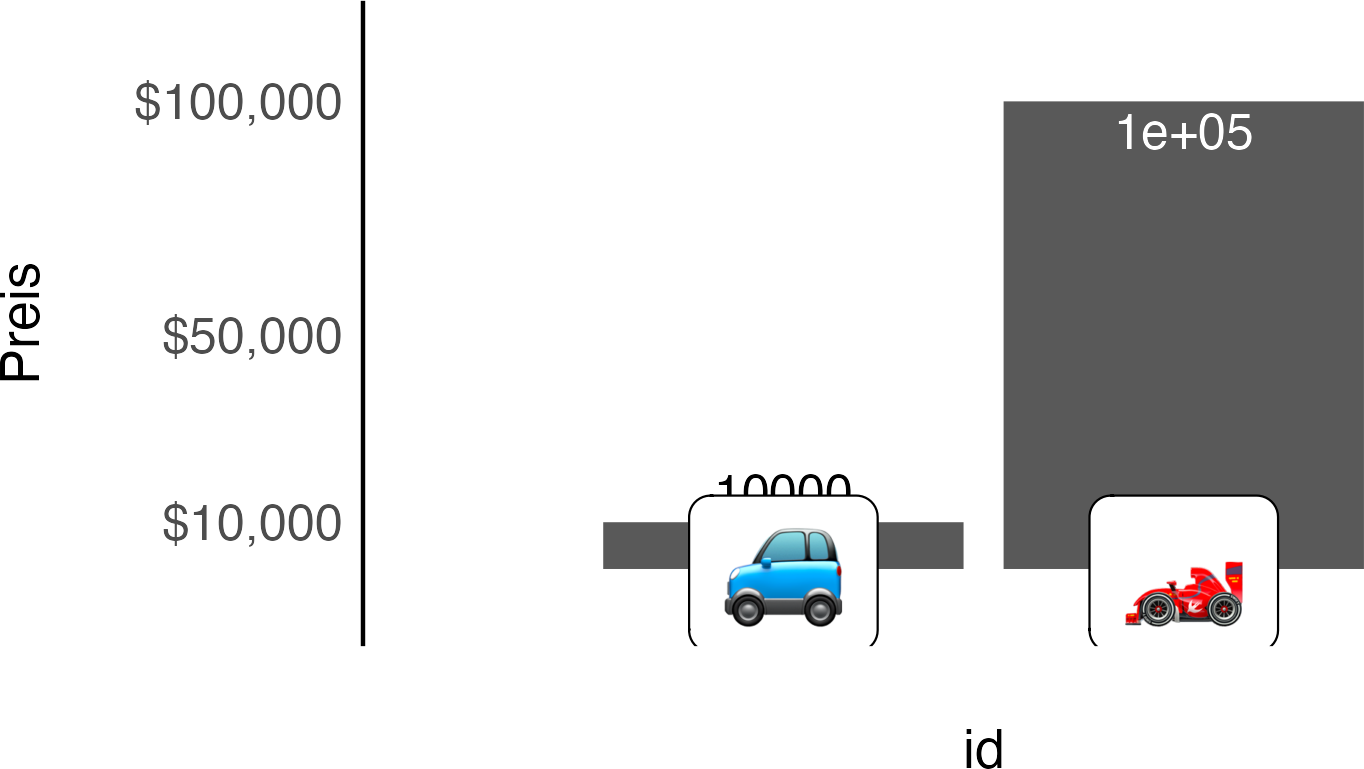
\includegraphics{010-rahmen_files/figure-pdf/fig-verhaeltnis-1.png}

}

\caption{\label{fig-verhaeltnis}Puh! Der rote Flitzer ist 10 Mal so
teuer wie die blaue Möhre. Kohlen zusammenkratzen.}

\end{figure}%

In \href{https://www.youtube.com/watch?v=_mN3kFe56ng}{diesem Video} gibt
es noch ausführlichere Erklärung zum Thema Skalenniveaus.

Außerdem können quantitative Variablen untergliedert werden in:

\begin{itemize}
\tightlist
\item
  \emph{stetige} Variablen, das sind Variablen, bei denen man zwischen
  zwei Ausprägungen immer noch eine weitere quetschen kann. So gibt es
  eine Wert für die Köpergröße zwischen 1.60\,m und 1.61\,m. Und einen
  Wert zwischen 1.601\,m und 1.602\,m, etc.
\item
  diskrete Variablen, das sind metrische Variablen, die nur bestimmte
  Ausprägungen haben, häufig sind das die natürlichen Zahlen:
  \(1,2,...\). Ein Beispiel wäre die Anzahl der Kinder in einer Familie.
\end{itemize}

\begin{tcolorbox}[enhanced jigsaw, toptitle=1mm, rightrule=.15mm, colbacktitle=quarto-callout-tip-color!10!white, breakable, title=\textcolor{quarto-callout-tip-color}{\faLightbulb}\hspace{0.5em}{Tipp}, bottomrule=.15mm, colback=white, opacitybacktitle=0.6, left=2mm, titlerule=0mm, toprule=.15mm, coltitle=black, opacityback=0, bottomtitle=1mm, arc=.35mm, leftrule=.75mm, colframe=quarto-callout-tip-color-frame]

Fragen nach Skalenniveaus gehören zu den Lieblingsprüfungsfragen in
diesem Themenbereich. Sie sind gut beraten, sich gerade mit dieser Frage
intensiver zu beschäftigen. Auch in thematisch angrenzenden Fächern wird
immer wieder die Frage nach dem Skalennvieau aufgeworfen. Das zeigt
natürlich auch die hohe Relevanz des Themas.

\end{tcolorbox}

\begin{exercise}[]\protect\hypertarget{exr-skalenniveaus}{}\label{exr-skalenniveaus}

Überlegen Sie sich für einige Variablen die Skalenniveaus und befragen
Sie dann eine:n Kommilitonen dazu. \(\square\)

\end{exercise}

\section{Modelle}\label{modelle}

Woran denken Sie beim Wort ``Modell''? Vielleicht an Spielzeugautos, s.
Abbildung~\ref{fig-matchbox}.

\begin{figure}

\centering{

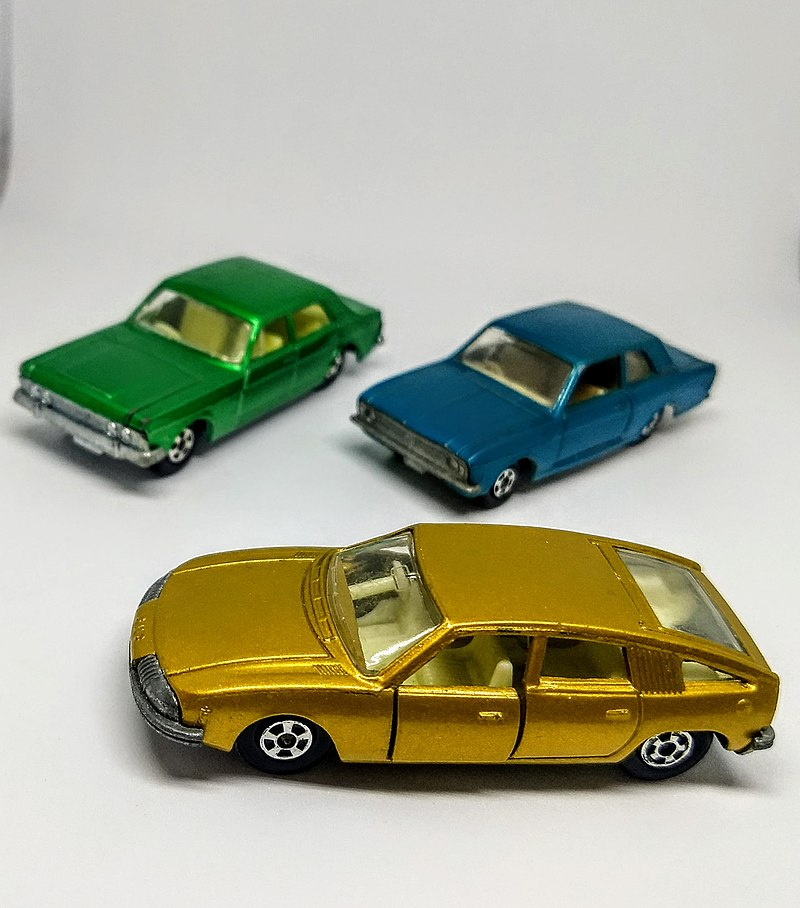
\includegraphics[width=0.25\textwidth,height=\textheight]{img/matchbox.jpg}

}

\caption{\label{fig-matchbox}Matchbox-Autos sind Modelle für Autos}

\end{figure}%

\begin{definition}[Modelle]\protect\hypertarget{def-modelle}{}\label{def-modelle}

Modelle sind ein vereinfachtes Abbild der Realität eine
\emph{Repräsentation} (Kaplan, 2009).\(\square\)

\end{definition}

\begin{example}[Beispiele für
Modelle]\protect\hypertarget{exm-Modelle}{}\label{exm-Modelle}

Puppen sind Modelle für Babies, Landkarten für Landstriche und
\href{https://de.wikipedia.org/wiki/Bohrsches_Atommodell}{das Atommodell
von Nils Bohr} ist ein Modell für Atome.\(\square\)

\end{example}

Auch in der Statistik nutzen wir Modelle. Helfen Sie Prof.~Weiss-Ois: Er
blickt nicht durch. Gerne würde er wissen, wie viele Stunden seine
Studentis auf die Prüfung lernen. Aber mit so vielen Zahlen kann er
nicht umgehen \ldots{} Geben Sie ihm ein Modell: Sagen Sie ihm, wie lang
die Studis typischerweise lernen (sagen Sie ihm ein einfach den
Mittelwert der Lernzeiten).

\begin{figure}

\begin{minipage}{0.50\linewidth}

\section{Vorher}\label{vorher-1}

12, 8, 10, 11, 10, 9, 13, 9, 14, 9, 12, 14, 7, 9, 9, 11, 9, 4, 5, 12, 9,
6, 9, 12, 13, 9, 9, 6, 10, 8


\includegraphics[width=0.25\textwidth,height=\textheight]{img/teacher.png}

\subcaption{\label{firstcol}Oh jeh, so viele Zahlen! Ich check nix! Wie
viel lernen denn jetzt meine Studis?!}
\end{minipage}%
%
\begin{minipage}{0.50\linewidth}

\section{Nachher}\label{nachher-1}

\textbf{9.6}


\includegraphics[width=0.25\textwidth,height=\textheight]{img/teacher.png}

\subcaption{\label{secondcol}Yeah, jetzt weiß ich, wie viel die Studis
so typischerweise lernen. Viel zu wenig natürlich!}
\end{minipage}%

\end{figure}%

\href{https://www.flaticon.com/free-icons/professor}{Icon unter Flaticon
licence, Autor: iconixar}

Der Nutzen von Modellen ist, dass sie komplexe Sachverhalte vereinfachen
und damit oft überhaupt erst dem Verständnis oder einer Untersuchung
zugänglich machen: Modelle ermöglichen Verständnis. In der Datenanalyse
bzw. Statistik\footnote{die beiden Begriffe werden hier weitgehend
  synonym gebraucht} fassen Sie oft viele Daten prägnant zusammen, z.B.
zu einer einzelnen Kennzahl. Das Verrückte an Modellen ist, dass man
Informationen wegwirft, um eine (andere, hoffentlich nützlichere)
Information zu bekommen (Stigler, 2016). Weniger ist mehr?!

\section{Praxisbezug}\label{praxisbezug}

Wir leben im Datenzeitalter; Daten durchdringen alle Bereiche des
beruflichen, gesellschaftlichen und privaten Lebens. Die Datenanalyse
hat sich in den letzten Jahren massiv verändert, s.
Abbildung~\ref{fig-fo-früher-heute}.

\begin{figure}

\centering{

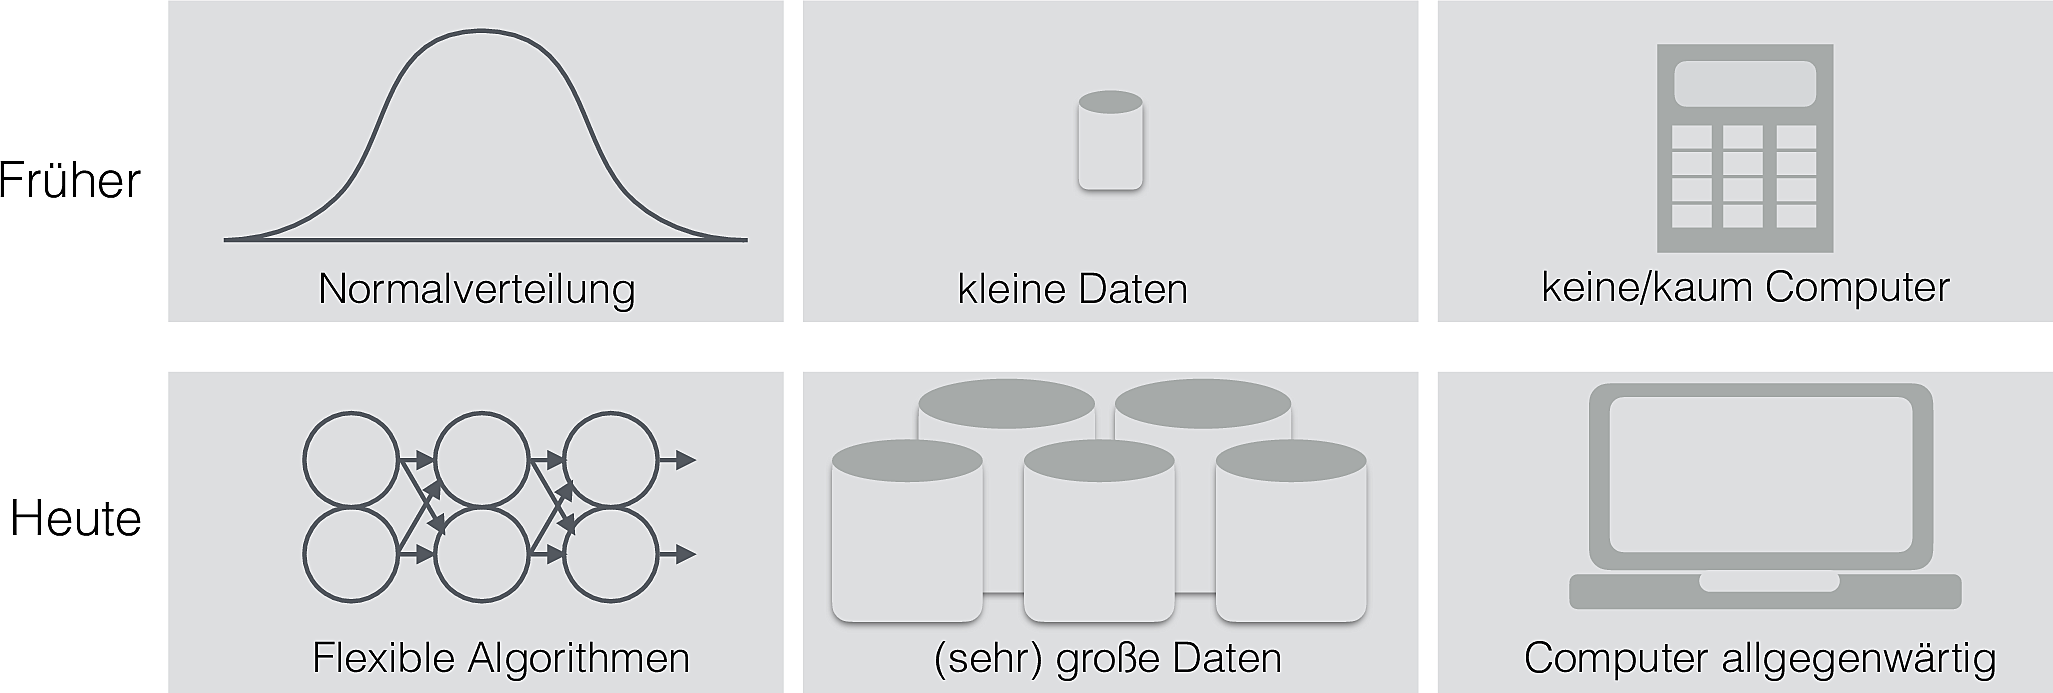
\includegraphics{img/Forschung_frueher_heute-crop.png}

}

\caption{\label{fig-fo-früher-heute}Forschung früher und heute}

\end{figure}%

Diese Entwicklung ist durchaus auch kritisch zu betrachten. Mit der
wachsenden Bedeutung von Daten wächst in gleichem Maße die Bedeutung von
Datenanalyse. Denn Daten ohne Sinn sind nutzlos. Aus diesem Grund kann
man sagen, dass Datenanalyse (und damit auch Statistik als eine
spezielle Art von Datenanalyse) zu stark nachgefragten Jobs gehören.

Laut \href{https://web.arbeitsagentur.de/entgeltatlas/beruf/129987}{dem
Entgeltatlas der Bundesagentur für Arbeit} liegt ein typisches Gehalt
von Data Scientisten bei knapp 6000 € pro Monat (in der Altersgruppe von
25 bis 54)\footnote{Abrufdatum: 1.2.23}. Laut dem
\href{https://gehaltsreporter.de/gehaelter-von-a-bis-z/it/data-scientist/}{Gehaltsreporter}
liegt das Einstiegsgehalt dieser Berufsgruppe bei knapp 50.000€ pro
Jahr.

\section{Fazit}\label{fazit}

Die Aufgabe von Statistik ist es, durch Zusammenfassen von Daten Modelle
zu bilden, die es uns einfacher machen, schwierige Sachverhalte zu
verstehen. Zentral ist dabei, die Analyse von Variabilität der Daten.
Daten kommen in verschiedenen Varianten vor, typischerweise in
Tabellenform, möglichst im Tidy-Format.

\section{Aufgaben}\label{aufgaben}

\begin{enumerate}
\def\labelenumi{\arabic{enumi}.}
\tightlist
\item
  \href{https://datenwerk.netlify.app/posts/variation01/variation01.html}{variation01}
\item
  \href{https://datenwerk.netlify.app/posts/def-statistik01/def-statistik01}{Def-Statistik01}
\item
  \href{https://datenwerk.netlify.app/posts/tidy1/tidy1.html}{tidy1}
\item
  \href{https://datenwerk.netlify.app/posts/skalenniveau1a/skalenniveau1a}{Skalenniveau1a}
\item
  \href{https://datenwerk.netlify.app/posts/ziele-statistik/ziele-statistik}{Ziele-Statistik}
\item
  \href{https://datenwerk.netlify.app/posts/variation02/variation02.html}{variation02}
\item
  \href{https://datenwerk.netlify.app/posts/skalenniveau1b/skalenniveau1b}{Skalenniveau1b}
\item
  \href{https://datenwerk.netlify.app/posts/tidydata1/tidydata1.html}{tidydata1}
\end{enumerate}

\section{Vertiefung}\label{vertiefung}

Fassen Sie den Artikel von Broman \& Woo (2018) zusammen.

Inspiration von einer Praktikerin der Datenanalyse: Caitlin Hudon verrät
\href{https://www.youtube.com/watch?v=O5lP6XcopdQ&list=PL9HYL-VRX0oQchs7dqFICoxMgnvFO10tC&index=15&t=1s}{in
diesem Video}, welche Fehler Sie sie in in den acht Jahren ihrer
Berufserfahrung gemacht hat und was sie daraus gelernt hat.

\url{https://www.youtube.com/watch?v=O5lP6XcopdQ&list=PL9HYL-VRX0oQchs7dqFICoxMgnvFO10tC&index=15&t=1s}

\section{Literaturhinweise}\label{literaturhinweise}

Einen Einblick in die Fundamente statistischer Analyse bietet Stigler
(2016). Çetinkaya-Rundel \& Hardin (2021), stellen grundlegende Konzepte
der Analyse von Daten im Kapitel 1, ``Hello data'', vor. Downey (2023)
illustriert statistische Überraschungsmoment auf unterhaltsame, und vor
allem: sofataugliche Art.

\section*{Literatur}\label{literatur-1}
\addcontentsline{toc}{section}{Literatur}

\phantomsection\label{refs}
\begin{CSLReferences}{1}{0}
\bibitem[\citeproctext]{ref-broman_data_2018}
Broman, K. W., \& Woo, K. H. (2018). Data Organization in Spreadsheets.
\emph{The American Statistician}, \emph{72}(1), 2--10.
\url{https://doi.org/10.1080/00031305.2017.1375989}

\bibitem[\citeproctext]{ref-cetinkaya-rundel_introduction_2021-1}
Çetinkaya-Rundel, M., \& Hardin, J. (2021). \emph{Introduction to Modern
Statistics. {OpenIntro}.} OpenIntro.
\url{https://openintro-ims.netlify.app/}

\bibitem[\citeproctext]{ref-downey_probably_2023}
Downey, A. (2023). \emph{Probably Overthinking It: How to Use Data to
Answer Questions, Avoid Statistical Traps, and Make Better Decisions}.
The University of Chicago Press.

\bibitem[\citeproctext]{ref-world_economic_forum_future_2020}
Forum, W. E. (2020). \emph{The {Future} of {Jobs Report} 2020}. World
Economic Forum.
\url{https://www3.weforum.org/docs/WEF_Future_of_Jobs_2020.pdf}

\bibitem[\citeproctext]{ref-kaplan_statistical_2009}
Kaplan, D. T. (2009). \emph{Statistical Modeling: A Fresh Approach}.
CreateSpace. \url{https://dtkaplan.github.io/SM2-bookdown/}

\bibitem[\citeproctext]{ref-poldrack_statistical_2023}
Poldrack, R. A. (2023). \emph{Statistical Thinking: Analyzing Data in an
Uncertain World}. Princeton University Press.
\url{https://statsthinking21.github.io/statsthinking21-core-site/}

\bibitem[\citeproctext]{ref-rothstein_publication_2014}
Rothstein, H. R. (2014). Publication {Bias}. In \emph{Wiley {StatsRef}:
{Statistics Reference Online}}. John Wiley \& Sons, Ltd.
\url{https://doi.org/10.1002/9781118445112.stat07071}

\bibitem[\citeproctext]{ref-schwaiger_impact_2022}
Schwaiger, E., \& Tahir, R. (2022). The Impact of Nomophobia and
Smartphone Presence on Fluid Intelligence and Attention.
\emph{Cyberpsychology: Journal of Psychosocial Research on Cyberspace},
\emph{16}(1). \url{https://doi.org/10.5817/CP2022-1-5}

\bibitem[\citeproctext]{ref-stigler_seven_2016}
Stigler, S. M. (2016). \emph{The Seven Pillars of Statistical Wisdom}.
Harvard University Press.

\bibitem[\citeproctext]{ref-ward_brain_2017}
Ward, A. F., Duke, K., Gneezy, A., \& Bos, M. W. (2017). Brain Drain:
{The} Mere Presence of One's Own Smartphone Reduces Available Cognitive
Capacity. \emph{Journal of the Association for Consumer Research},
\emph{2}(2), 140--154. \url{https://doi.org/10.1086/691462}

\bibitem[\citeproctext]{ref-wickham_r_2018}
Wickham, H., \& Grolemund, G. (2018). \emph{R Für Data Science: {Daten}
Importieren, Bereinigen, Umformen, Modellieren Und Visualisieren} (F.
Langenau, Übers.; 1. Auflage). O'Reilly.
\url{https://r4ds.had.co.nz/index.html}

\end{CSLReferences}



\end{document}
